%-------------------------------------------------------------------------------
%                                PREAMBLE
%-------------------------------------------------------------------------------
\documentclass[usenames,dvipsnames,svgnames,10pt,aspectratio=169]{beamer}
%
\usefonttheme{professionalfonts}
% This theme uses TIKZ: compile twice with PDFLaTeX or LuaLaTeX.
%
%  Options:
%  - [clean]:    clean slides, i.e. logos and footbar are removed
%  - [kth]:      footbar style inspierd to the official KTH template
%  - [nicewave]: a different style of wave is used (not approved by FLOW)
%
\usetheme[kth]{flow}

\usepackage{hyperref,graphicx,lmodern}
\usepackage[utf8]{inputenc}
\usepackage{media9}
\usepackage{xcolor}
\usepackage{stmaryrd}
\usepackage{nicefrac}
\usepackage{multimedia}
\usepackage{multicol}
\usepackage{upgreek}
\usepackage[]{bm}
\usepackage[]{url}
\usepackage[]{animate}
\usepackage{amsmath}
\usepackage[]{listings}

\graphicspath{{imgs/}}
\setbeamertemplate{blocks}[rounded][shadow=true]

\usepackage{listings}
\usepackage{textgreek}

\lstset{
	basicstyle=\small\ttfamily,
	columns=fullflexible, % make sure to use fixed-width font, CM typewriter is NOT fixed width
	% numbers=false,
	numberstyle=\small\ttfamily\color{Gray},
	stepnumber=1,
	numbersep=10pt,
	numberfirstline=false,
	numberblanklines=false,
	tabsize=4,
	lineskip=-1.5pt,
	extendedchars=true,
	breaklines=true,
	keywordstyle=\color{Blue}\bfseries,
	identifierstyle=, % using emph or index keywords
	commentstyle=\sffamily\color{OliveGreen},
	stringstyle=\color{Maroon},
	showstringspaces=false,
	showtabs=false,
	upquote=false,
	texcl=true % interpet comments as LaTeX
}

\lstdefinelanguage{julia}
{
  keywordsprefix=\@,
  morekeywords={
    exit,whos,edit,load,is,isa,isequal,typeof,tuple,ntuple,uid,hash,finalizer,convert,promote,
    subtype,typemin,typemax,realmin,realmax,sizeof,eps,promote_type,method_exists,applicable,
    invoke,dlopen,dlsym,system,error,throw,assert,new,Inf,Nan,pi,im,begin,while,for,in,return,
    break,continue,macro,quote,let,if,elseif,else,try,catch,end,bitstype,ccall,do,using,module,
    import,export,importall,baremodule,immutable,local,global,const,Bool,Int,Int8,Int16,Int32,
    Int64,Uint,Uint8,Uint16,Uint32,Uint64,Float32,Float64,Complex64,Complex128,Any,Nothing,None,
    function,type,typealias,abstract
  },
  sensitive=true,
  morecomment=[l]{\#},
  morestring=[b]',
  morestring=[b]"
}
%-------------------------------------------------------------------------------
%                                TITLE PAGE
%-------------------------------------------------------------------------------
\title[Nonlinear physics] % Short title used in footline
{
	Nonlinear physics, dynamical \\
	systems and chaos theory
}

\author[J.-Ch.~Loiseau] % Presenting author in short form used in footline
{
	\underline{Jean-Christophe Loiseau}
}
% - Give the names in the same order as the appear in the paper.
% - Underline the presenting author.

\institute[unused]
{
	\url{jean-christophe.loiseau@ensam.eu} \\
	Laboratoire DynFluid \\
	Arts et M\'etiers, France.
}
% Keep it simple, no one is interested in your street address.

% University logo(s)
\logot{
\includegraphics[width=.128\paperwidth]{DynFluid_logo}}  % Top logo
\logob{
\includegraphics[width=0.128\paperwidth]{ENSAM_logo}} % Bottom logo
% \logoc[{\includegraphics[width=.128\paperwidth]{limsi}}]{\includegraphics[width=.128\paperwidth]{limsi}} % Corner logo
%
% Cover image: \cvrimg{x position}{y position}{cover image}
\cvrimg{.77}{.8}{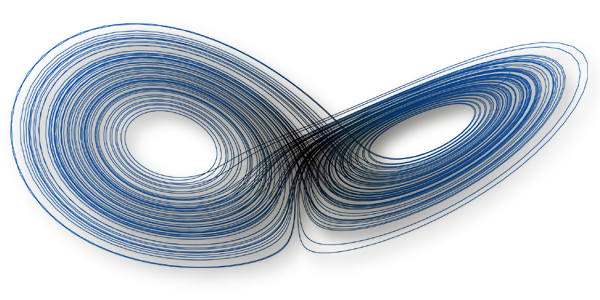
\includegraphics[width=.4\paperwidth]{cover.png}}

\date[unused]{Physique non-lin\'eaire -- 2019-2020}

\begin{document}

\titleframe	% Print the title as the first slide

%-------------------------------------------------------------------------------
%                           PRESENTATION SLIDES
%-------------------------------------------------------------------------------

\begin{frame}[t, c]{One-dimensional maps}{Introduction}
	\begin{minipage}{.58\textwidth}
		\begin{itemize}
			\item Let us focus our attention onto \emph{discrete-time systems}.
			\begin{itemize}
				\item[\( \hookrightarrow \)] Also known as difference equations, recursion relations, iterated maps or simply maps.
			\end{itemize}

			\medskip

			\item Maps arise in various ways:
			\begin{itemize}
				\item[\( \hookrightarrow \)] Tools for analyzing differential equations (see Poincarré and Lorenz maps).
				\item[\( \hookrightarrow \)] Models of natural phenomena (e.g.\ digital electronics, finance).
				\item[\( \hookrightarrow \)] As simple examples of chaos (what we'll do today).
			\end{itemize}

			\medskip

			\item We'll focus on one-dimensional maps for now.
			\begin{itemize}
				\item[\( \hookrightarrow \)] Easy and fast to simulate on a computer.
			\end{itemize}
		\end{itemize}
	\end{minipage}%
	\hfill
	\begin{minipage}{.38\textwidth}
		\centering
		\begin{block}{\centering \textbf{Logistic map}}
			\centering
			\( x_{k+1} = \mu x_k \left( 1 - x_k \right) \)
		\end{block}

		\begin{block}{\centering \textbf{Sine map}}
			\centering
			\( x_{k+1} = \mu \sin \left( \pi x_k \right) \)
		\end{block}

		\begin{block}{\centering \textbf{Tent map}}
			\centering
			\[
				x_{k+1} = \begin{cases}
										\mu x \quad 0 \leq x \leq \nicefrac{1}{2} \\
										\mu - \mu x \quad \nicefrac{1}{2} \leq x \leq 1.
									\end{cases}
			\]
		\end{block}

	\end{minipage}

	\vspace{1cm}
\end{frame}

\begin{frame}[t, c]{One-dimensional maps}{Introduction}
	\centering

	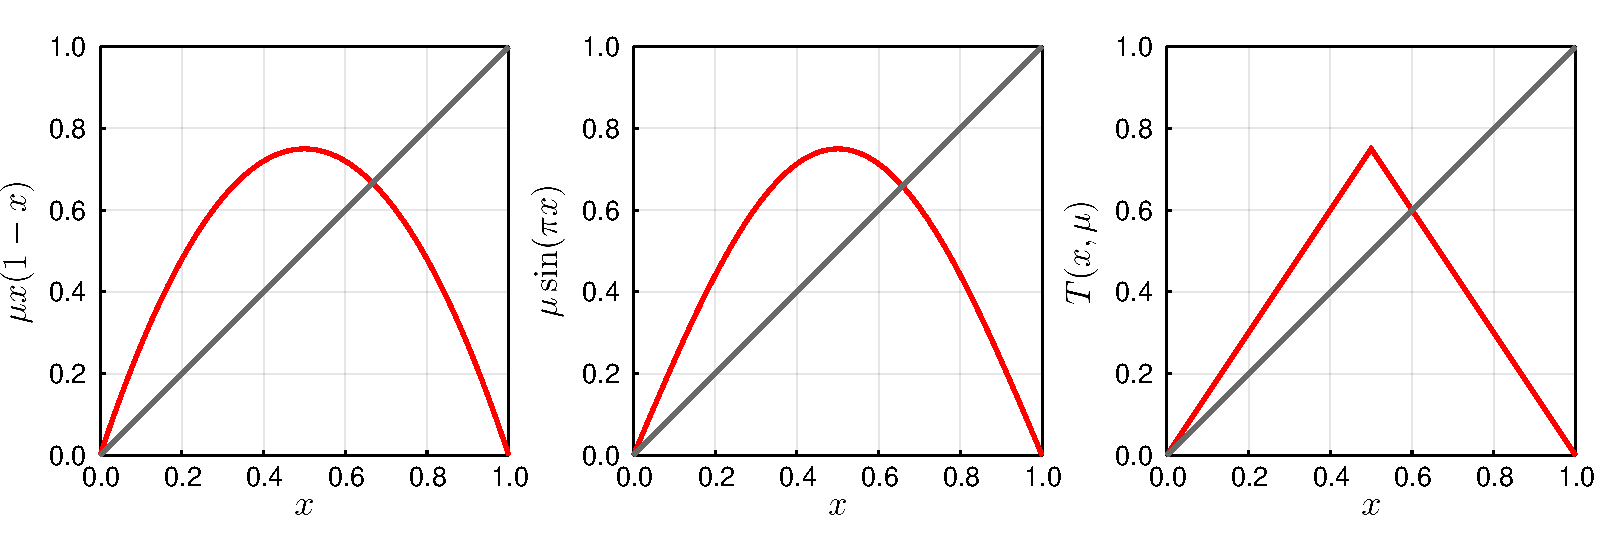
\includegraphics[width=.8\textwidth]{1D_maps_introduction}

	\vspace{1cm}
\end{frame}

\begin{frame}[t, c]{One-dimensional maps}{Fixed points and cobwebs}
	\begin{minipage}{.68\textwidth}
		\begin{itemize}
			\item Fixed points satisfy the equation
			%
			\[
				x^* = f(x^*).
			\]

			\item Their stability is governed by the asymptotic fate of an infinitesimal perturbation \( \eta \) whose dynamics are governed by
			%
			\[
				\eta_{k+1} = f^{\prime}(x^*) \eta_k + \mathcal{O}\left( \eta_k^2 \right).
			\]

			\item Neglecting the higher-order terms, we end up with the \emph{linearized equation}
			%
			\[
				\eta_{k+1} = f^{\prime} \left( x^* \right) \eta_k.
			\]
		\end{itemize}
	\end{minipage}%
	\hfill
	\begin{minipage}{.28\textwidth}
		\centering
		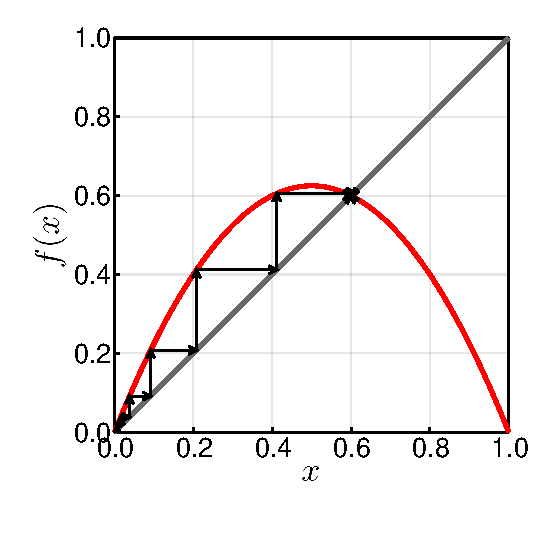
\includegraphics[width=\textwidth]{cobweb_logistic_map}
	\end{minipage}

	\vspace{1cm}
\end{frame}

\begin{frame}[t, c]{One-dimensional maps}{Fixed points and cobwebs}
	\begin{minipage}{.68\textwidth}
		\begin{itemize}
			\item Introducing \( \lambda = f^{\prime} \left( x^* \right) \), the solution to the linearized equation is
			%
			\[
				\eta_{k+1} = \lambda^k \eta_0.
			\]

			\item If \( \vert \lambda \vert < 1 \), then \( \eta_{k} \to 0 \) as \( k \to \infty \).
			The fixed point is \textbf{linearly stable}.

			\medskip

			\item If \( \vert \lambda \vert > 1 \), then \( \eta_{k} \to \infty \) as \( k \to \infty \).
			The fixed point is \textbf{linearly unstable}.

			\medskip

			\item If \( \vert \lambda \vert = 1 \), the fixed point is \textbf{marginally stable} and the higher-order terms can no longer be neglected.
		\end{itemize}
	\end{minipage}%
	\hfill
	\begin{minipage}{.28\textwidth}
		\centering
		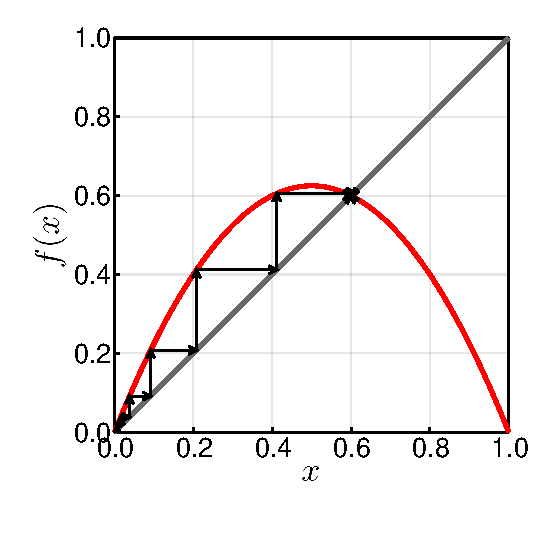
\includegraphics[width=\textwidth]{cobweb_logistic_map}
	\end{minipage}

	\vspace{1cm}
\end{frame}

\begin{frame}[t, c]{Logistic map}{Introduction}
	\begin{minipage}{.68\textwidth}
		\begin{itemize}
			\item Used by Robert May (1976) to illustrate how simple nonlinear maps can have very complicated dynamics.

			\medskip

			\item Article ends with \emph{an evangelical plea for the introduction of these difference equations into elementary mathematics courses so that students' intuition may be enriched by seeing the wild thing that simple nonlinear equations can do.}
		\end{itemize}
	\end{minipage}%
	\hfill
	\begin{minipage}{.28\textwidth}
		\centering
		\begin{block}{\centering \textbf{Logistic map}}
			\centering
			\(	x_{k+1} = \mu x_k \left( 1 - x_k \right) \)
		\end{block}
	\end{minipage}

	\vspace{1cm}
\end{frame}

\begin{frame}[t, c]{Logistic map}{Numerics}
	\begin{minipage}{.38\textwidth}
		\centering
		\lstinputlisting[language=Julia]{example.jl}
	\end{minipage}%
	\hfill
	\begin{minipage}{.58\textwidth}
		\begin{itemize}
			\item Easy to simulate whichever programming language you use.

			\bigskip

			\item In the rest, we'll use the \texttt{DynamicalSystems.jl} package in \texttt{Julia}.
			\begin{itemize}
				\item[\( \hookrightarrow \)] 1\textsuperscript{st} place in the 2018 Software Contest held by the dynamical systems division of SIAM.

				\item[\( \hookrightarrow \)] Provides numerous tools to analyze dynamical systems.
			\end{itemize}

			\medskip

			\item Check Youtube and Jupyter tutorials if you want to start using this library.
		\end{itemize}
	\end{minipage}

	\vspace{1cm}
\end{frame}

\begin{frame}[t, c]{Logistic map}{Dynamics}
	\centering
	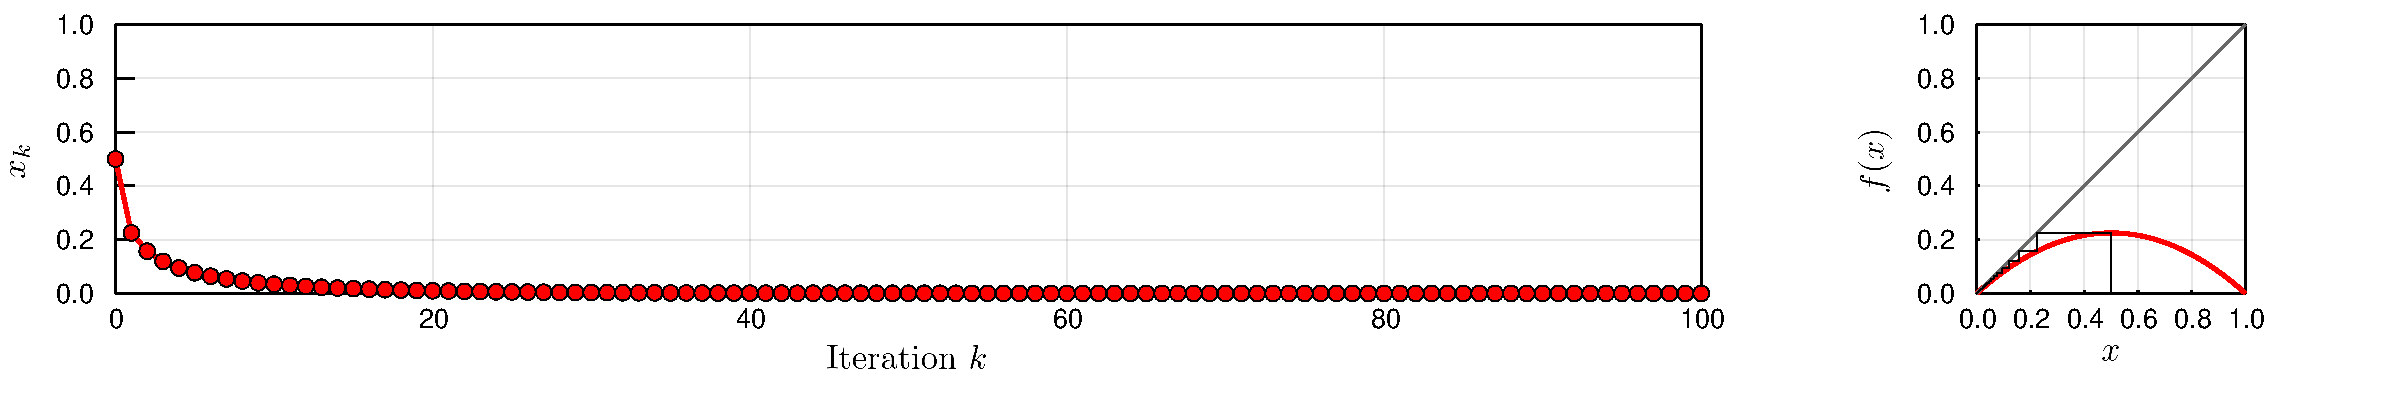
\includegraphics[width=\textwidth]{dynamics_a} \\
	{
	\small
	Dynamics for \( \mu = 0.9 \).
	}

	\begin{itemize}
		\item For small growth rate (\( r < 1\)), the population goes extinct.
	\end{itemize}

	\vspace{1cm}
\end{frame}

\begin{frame}[t, c]{Logistic map}{Dynamics}
	\centering
	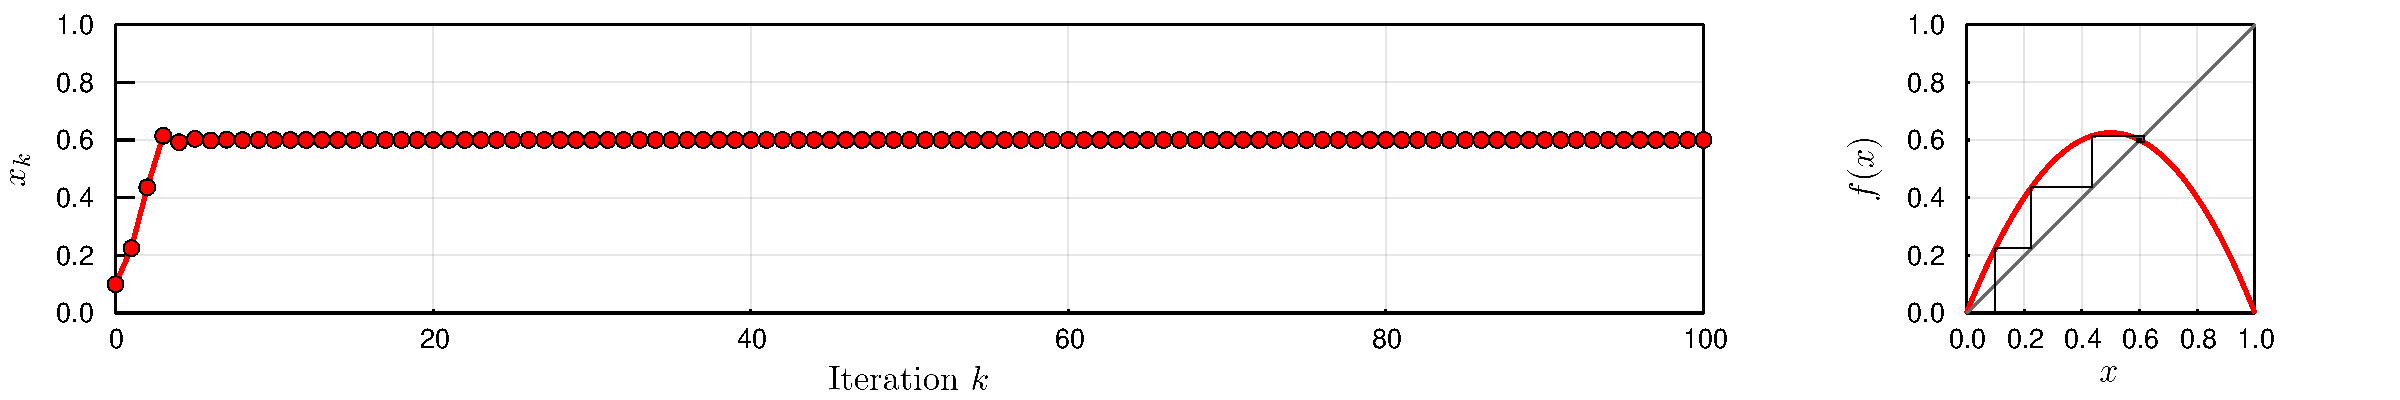
\includegraphics[width=\textwidth]{dynamics_b} \\
	{
	\small
	Dynamics for \( \mu = 2.5 \).
	}

	\begin{itemize}
		\item For \( 1 < r < 3 \), the population rows and eventually reaches a nonzero steady state.
	\end{itemize}

	\vspace{1cm}
\end{frame}

\begin{frame}[t, c]{Logistic map}{Dynamics}
	\centering
	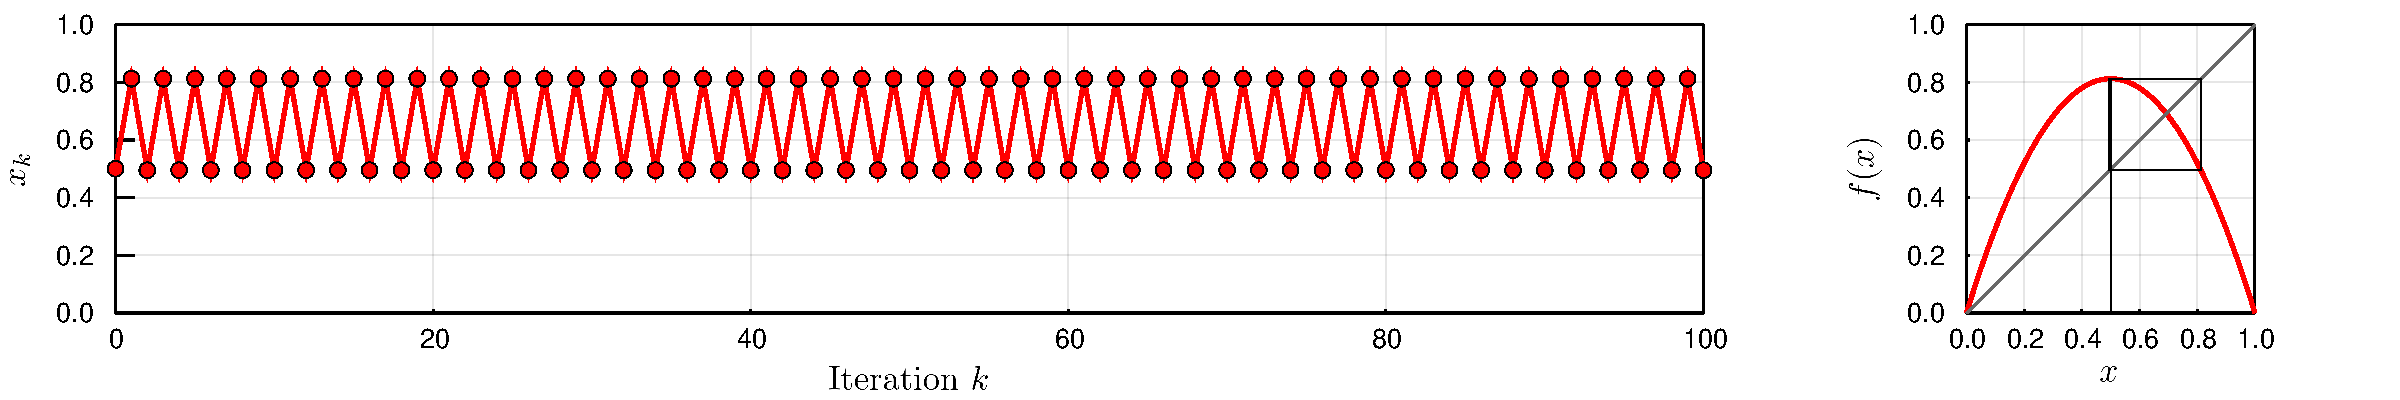
\includegraphics[width=\textwidth]{dynamics_c} \\
	{
	\small
	Dynamics for \( \mu = 3.25 \).
	}

	\begin{itemize}
		\item For larger \( \mu	\), the population oscillates periodically between two values.
		We have a \textbf{period-2} cycle.
	\end{itemize}

	\vspace{1cm}
\end{frame}

\begin{frame}[t, c]{Logistic map}{Dynamics}
	\centering
	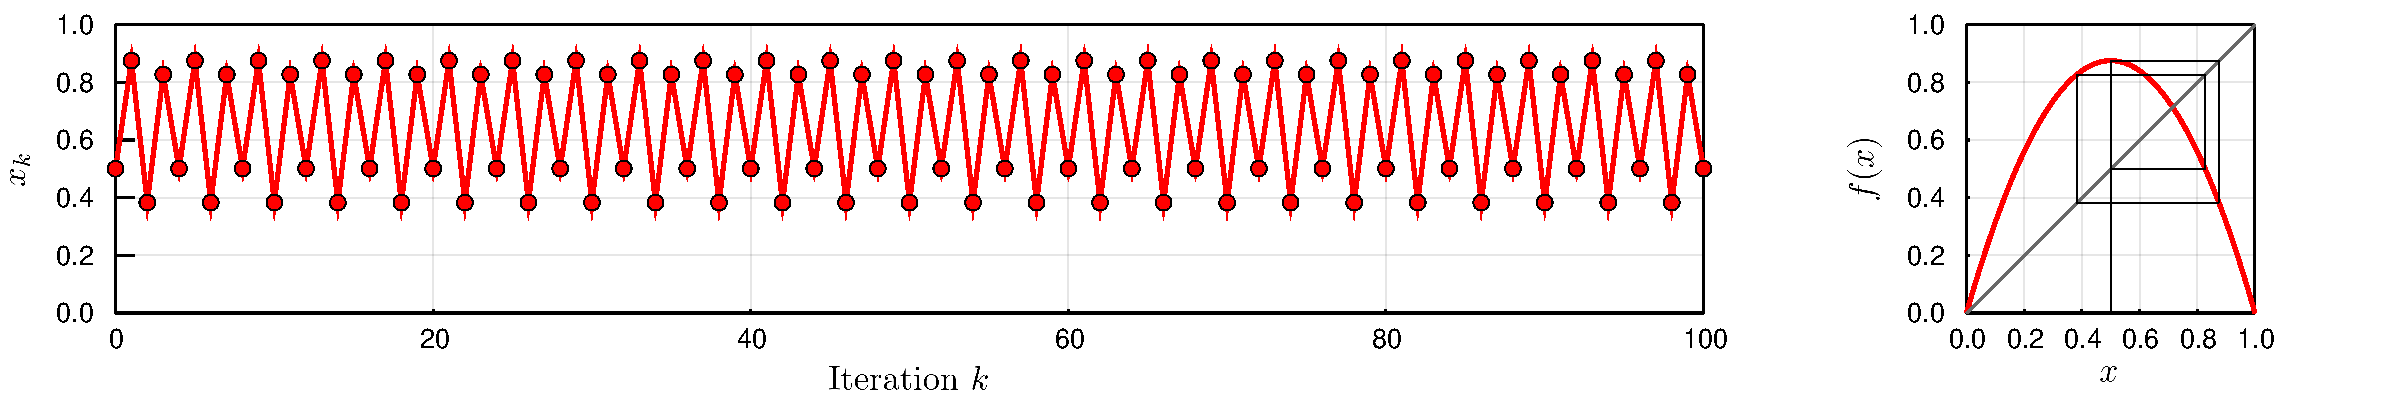
\includegraphics[width=\textwidth]{dynamics_d} \\
	{
	\small
	Dynamics for \( \mu = 3.5 \).
	}

	\begin{itemize}
		\item Further increasing \( \mu	\), the population oscillates between four values.
		We have a \textbf{period-4} cycle.
	\end{itemize}

	\vspace{1cm}
\end{frame}

\begin{frame}[t, c]{Logistic map}{Dynamics}
	\centering
	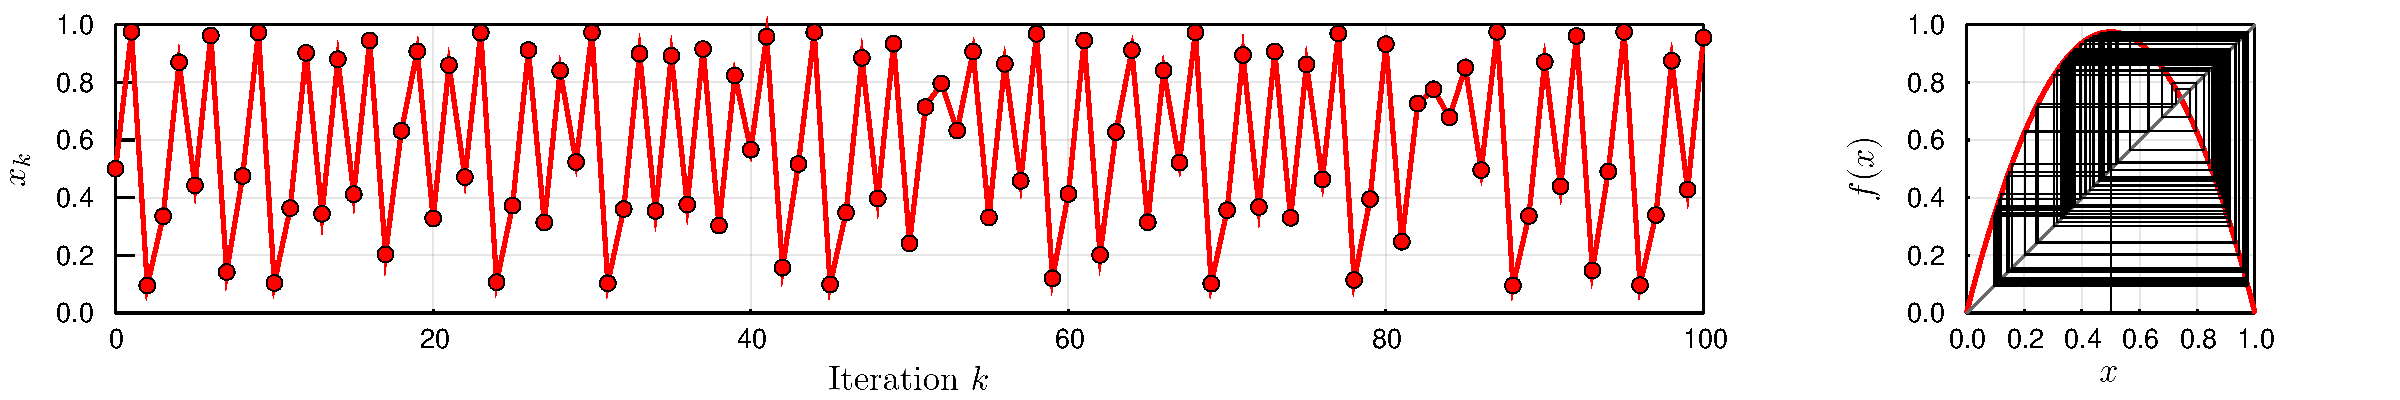
\includegraphics[width=\textwidth]{dynamics_e} \\
	{
	\small
	Dynamics for \( \mu = 3.9 \).
	}

	\begin{itemize}
		\item Finally, for \( \mu \) sufficiently large, the population behaves eratically.
		These are \textbf{chaotic dynamics}.
	\end{itemize}

	\vspace{1cm}
\end{frame}

\begin{frame}[t, c]{Logistic map}{Orbit diagram}
	\begin{minipage}{.48\textwidth}
		\begin{itemize}
			\item The evolution of the system's behaviour as \( \mu \) varies can be summarized in an \textbf{orbit diagram}.

			\medskip

			\item For the logistic map, the orbit diagram exhibits various features such as
			\begin{itemize}
				\item[\( \hookrightarrow \)] Fixed points,
				\item[\( \hookrightarrow \)] Bifurcations,
				\item[\( \hookrightarrow \)] 2\textsuperscript{n}-cycles,
				\item[\( \hookrightarrow \)] chaotic dynamics,
				\item[\( \hookrightarrow \)] \(3 \cdot 2\)\textsuperscript{n}-cycles,
				\item[\( \hookrightarrow \)] a fractal structure.
			\end{itemize}

			\medskip

			\item In the rest, we'll try to explain each of these.
		\end{itemize}
	\end{minipage}%
	\hfill
	\begin{minipage}{.48\textwidth}
		\centering
		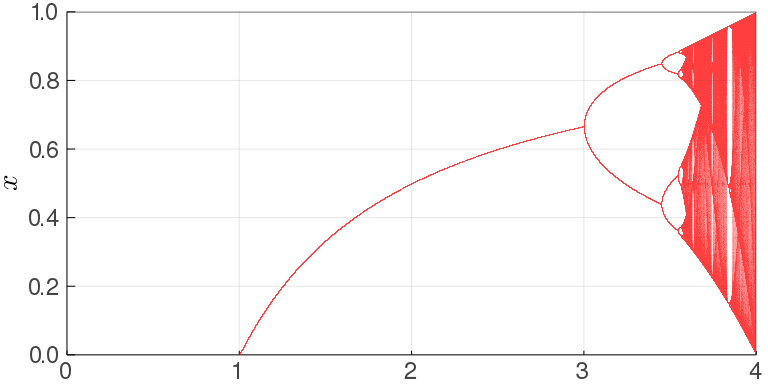
\includegraphics[width=\textwidth]{orbit_diagram_a}
	\end{minipage}

	\vspace{1cm}
\end{frame}

\begin{frame}[t, c]{Logistic map}{Analysis : Fixed points and stability}
	\begin{minipage}{.68\textwidth}
		\begin{itemize}
			\item Fixed points are solution to
			%
			\[
				\begin{aligned}
					& x = \mu	 x \left( 1 - x \right) \\
					& x \left( x - \frac{\mu -1}{\mu} \right) = 0.
				\end{aligned}
			\]

			\item It can easily be shown that the system admits the following fixed points:
			%
			\[
				\begin{aligned}
					& x^* = 0 \quad \forall \mu \in \left[ 0, 4 \right[, \\
					& x^* = \frac{\mu - 1}{\mu} \quad \forall 1 \leq \mu < 4.
				\end{aligned}
			\]
		\end{itemize}
	\end{minipage}%
	\hfill
	\begin{minipage}{.28\textwidth}
		\centering
		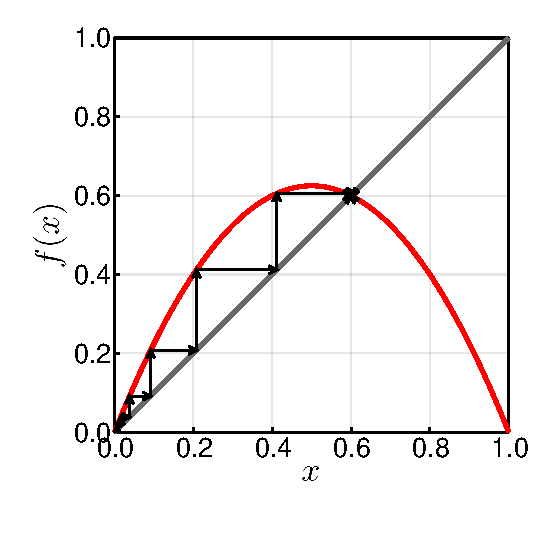
\includegraphics[width=\textwidth]{cobweb_logistic_map}
	\end{minipage}

	\vspace{1cm}
\end{frame}

\begin{frame}[t, c]{Logistic map}{Analysis : Fixed points and stability}
	\begin{minipage}{.68\textwidth}
		\begin{itemize}
			\item Fixed points are linearly stable if \( \vert f^{\prime}\left( x^*, \mu \right) \vert < 1 \) and linearly unstable if \( \vert f^{\prime}\left( x^*, \mu \right) \vert > 1 \).
			\begin{itemize}
				\item[\( \hookrightarrow \)] If \( \vert f^{\prime}\left( x^*, \mu \right) \vert = 1 \), the fixed point is marginally stable and one needs to study the effect of the nonlinear terms.
				\item[\( \hookrightarrow \)] If \( \vert f^{\prime}\left( x^*, \mu \right) \vert = 0 \), the fixed point is said to be \textbf{super-stable}.
			\end{itemize}

			\medskip

			\item For the logistic map, simply maths show that
			\begin{itemize}
				\item[\( \hookrightarrow \)] \( x^* = 0 \) is stable for \( 0 \leq \mu < 1 \) and unstable otherwise.
				\item[\( \hookrightarrow \)] \( x^* = \nicefrac{\mu - 1}{\mu} \) is stable for \( 1 \leq \mu \leq 3\) and unstable for \( 3 \geq \mu \).
				\item[\( \hookrightarrow \)] \( x^* = \nicefrac{\mu - 1}{\mu} \) is super-stable for \( \mu = 2 \) (and thus \( x^* = \nicefrac{1}{2} \)).
			\end{itemize}
		\end{itemize}
	\end{minipage}%
	\hfill
	\begin{minipage}{.28\textwidth}
		\centering
		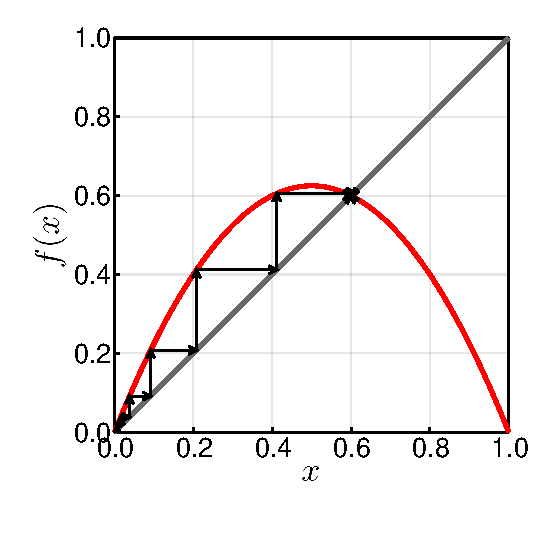
\includegraphics[width=\textwidth]{cobweb_logistic_map}
	\end{minipage}

	\vspace{1cm}
\end{frame}

\begin{frame}[t, c]{Logistic map}{Analysis : Stable and super-stable fixed points}
	\begin{minipage}{.68\textwidth}
		\begin{itemize}
			\item For a regular fixed point, we have seen that
			%
			\[
				\begin{aligned}
					\eta_{k+1} & = \lambda \eta_k + \mathcal{O}(\eta_k^2) \\
					& \simeq \lambda^k \eta_0.
				\end{aligned}
			\]

			\item For a superstable fixed point, \( \lambda = 0 \) and thus one can no longer neglect the quadratic term.
			Hence
			%
			\[
				\eta_{k+1} \sim \eta_0^{2^k}.
			\]

			\item Perturbations in the vicinity of a superstable fixed point decay much faster than they would in the vicinity of a regular fixed point.
		\end{itemize}
	\end{minipage}%
	\hfill
	\begin{minipage}{.28\textwidth}
		\centering
		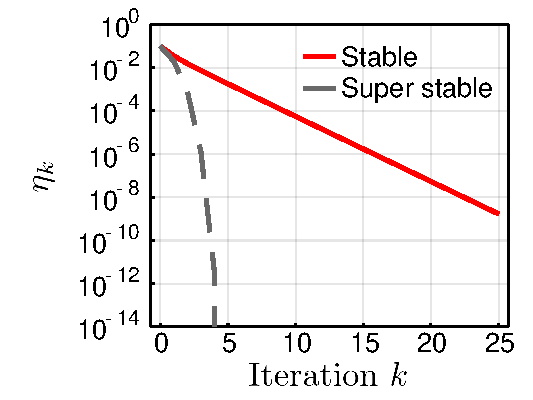
\includegraphics[width=\textwidth]{stable_vs_superstable}
	\end{minipage}

	\vspace{1cm}
\end{frame}

\begin{frame}[t, c]{Logistic map}{Analysis : Creation of a 2-cycle}
	\begin{minipage}{.68\textwidth}
		\begin{itemize}
			\item At \( \mu = 3\), \( x^* = \nicefrac{\mu-1}{\mu} \) looses its stability and \( f^{\prime}(x^*, \mu) = -1\).
			\begin{itemize}
				\item[\( \hookrightarrow \)] This is known as a \textbf{flip bifurcation} (or period-doubling).
				\item[\( \hookrightarrow \)] It gives rise to a 2-cycle.
			\end{itemize}
		\end{itemize}

		\medskip

		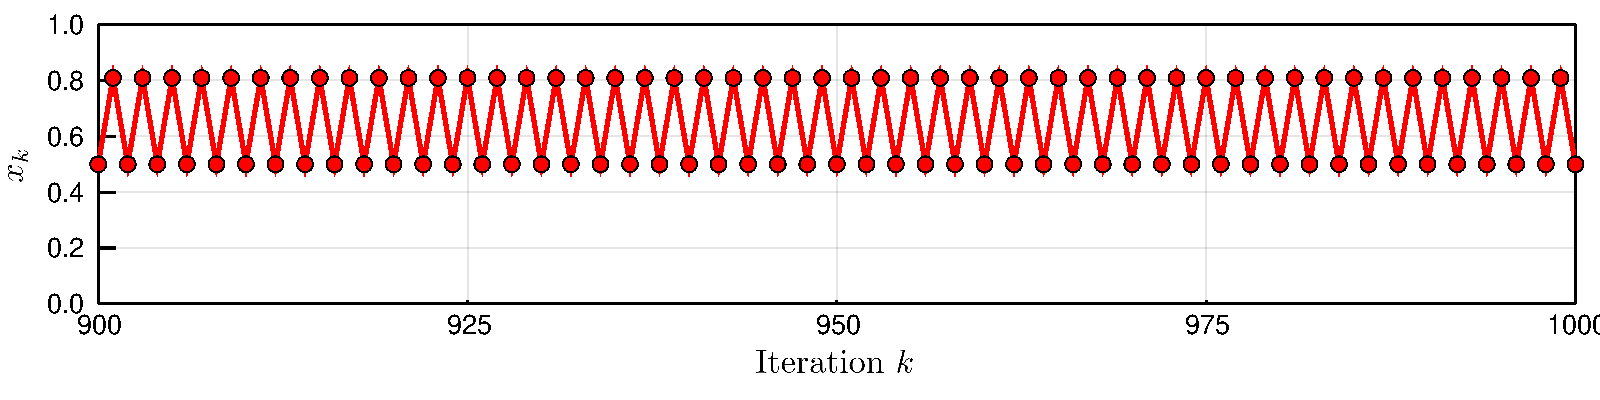
\includegraphics[width=\textwidth]{cycle_2_time_series}
	\end{minipage}%
	\hfill
	\begin{minipage}{.28\textwidth}
		\centering
		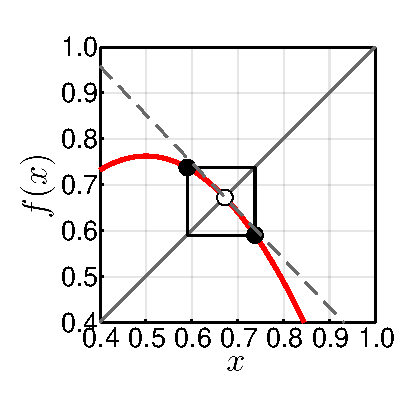
\includegraphics[width=\textwidth]{flip_bifurcation}
	\end{minipage}

	\vspace{1cm}
\end{frame}

\begin{frame}[t, c]{Logistic map}{Analysis : Creation of a 2-cycle}
	\begin{minipage}{.68\textwidth}
		\begin{itemize}
			\item The equations for a 2-cycle are
			%
			\[
				\begin{aligned}
					p & = f(q) \\
					q & = f(p).
				\end{aligned}
			\]

			\item Combining these two equations, \( p \) and \( q \) are thus fixed points of
			%
			\[
				f^2(x) - x = 0.
			\]

			\item For the logistic equation, we thus have
			%
			\[
				\mu^2 x \left( 1 - x \right) \left( 1 - \mu x \left( 1 - x \right) \right) = 0.
			\]
			%
			Factoring out \( x \) and \( x - \nicefrac{\mu -1}{\mu} \), we finally have
			%
			\[
				p, q = \frac{\mu + 1 \pm \sqrt{\left( \mu - 3 \right) \left( \mu + 1 \right)}}{2\mu}.
			\]
		\end{itemize}
	\end{minipage}%
	\hfill
	\begin{minipage}{.28\textwidth}
		\centering
		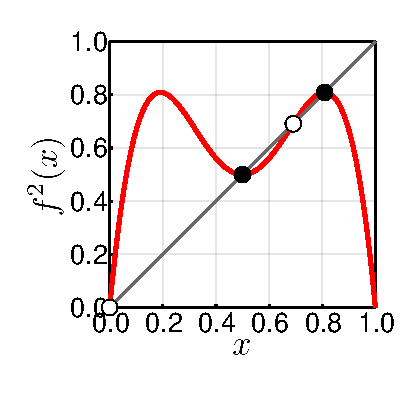
\includegraphics[width=\textwidth]{cycle_2_creation}
	\end{minipage}

	\vspace{1cm}
\end{frame}

\begin{frame}[t, c]{Logistic map}{Stability of a 2-cycle}
	\begin{minipage}{.68\textwidth}
		\begin{itemize}
			\item \( p \) and \( q \) being fixed points of \( x_{k+1} = f^2(x_k) \), their stability is dictated by
			%
			\[
				\begin{aligned}
					\lambda & = \displaystyle \frac{\mathrm{d}f^2(x)}{\mathrm{d}x} \Big\vert_{x=p} \\
					& = f^{\prime}(q) f^{\prime}(p) \\
					& = 4 + 2 \mu - \mu^2.
				\end{aligned}
			\]

			\item This 2-cycle is thus stable for
			%
			\[
				\vert 4 + 2\mu - \mu^2 \vert < 1,
			\]
			%
			i.e. for \( 3 < \mu < 1 + \sqrt{6} \ (= 3.449\ldots )\).

			\medskip

			\item It is superstable for \( \mu = 1 + \sqrt{5} \ (=3.236\ldots )\).
		\end{itemize}
	\end{minipage}%
	\hfill
	\begin{minipage}{.28\textwidth}
		\centering
		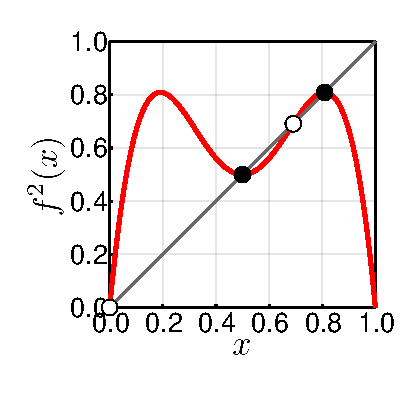
\includegraphics[width=\textwidth]{cycle_2_creation}
	\end{minipage}

	\vspace{1cm}
\end{frame}

\begin{frame}[t, c]{Logistic map}{Analysis : Creation of a 4-cycle}
	\begin{minipage}{.68\textwidth}
		\begin{itemize}
			\item At \( \mu = 1 + \sqrt{6} \), our 2-cycle looses its stability and \( \lambda = -1 \).
			\begin{itemize}
				\item[\( \hookrightarrow \)] As before, this is a period-doubling bifurcation.
				\item[\( \hookrightarrow \)] The system now exhibits a 4-cycle.
			\end{itemize}
		\end{itemize}

		\medskip

		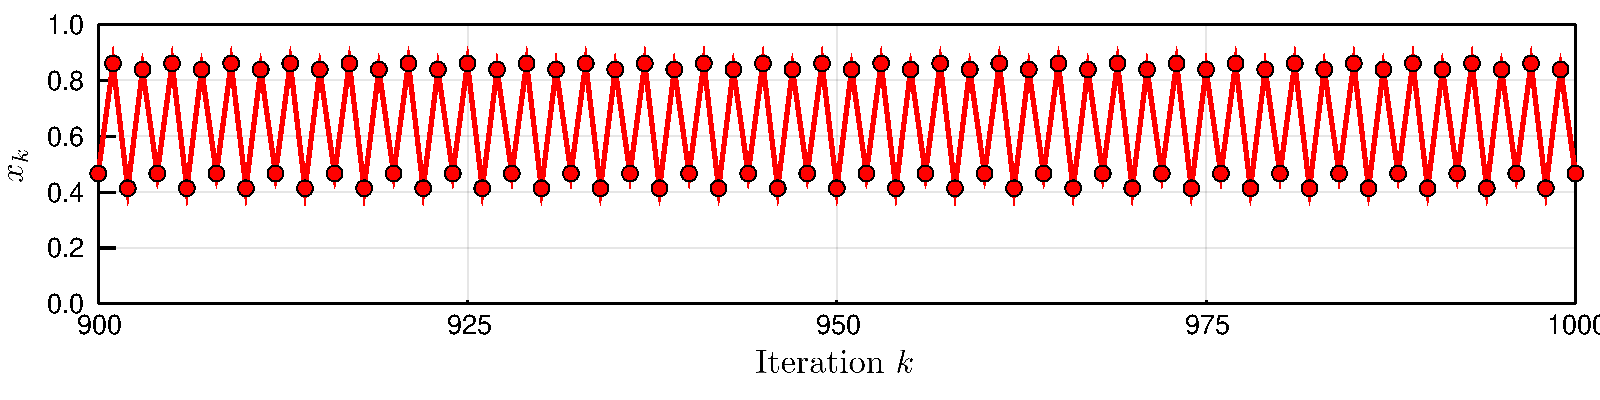
\includegraphics[width=\textwidth]{cycle_4_time_series}
	\end{minipage}%
	\hfill
	\begin{minipage}{.28\textwidth}
		\centering
		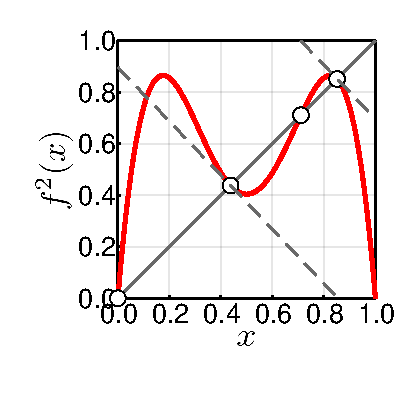
\includegraphics[width=\textwidth]{cycle_4_creation}
	\end{minipage}

	\vspace{1cm}
\end{frame}

\begin{frame}[t, c]{Logistic map}{Analysis : Subharmonic cascade}
	\begin{minipage}{.48\textwidth}
		\begin{itemize}
			\item We can generalize to \( 2^n \)-cycles.
			Points belonging to such cycles are fixed points of
			%
			\[
				f^{2^n}(x) - x = 0.
			\]

			\item Their stability is dictated by the modulus of
			%
			\[
				\lambda_n = \displaystyle \frac{\mathrm{d} f^{2^n}(x)}{\mathrm{d}x} \Big\vert_{x=p}.
			\]

			\item The critical parameter \( \mu_n \) for which \( \vert \lambda_n \vert = 1 \) needs to be evaluated numerically (for \( n > 2 \)).

			\medskip

			\item The sequence \( \left\{ \mu_n \right\}_{n=1, \infty} \) seems to converge as \( n \to \infty \) but to what value?
		\end{itemize}
	\end{minipage}%
	\hfill
	\begin{minipage}{.48\textwidth}
		\centering
		\begin{tabular}{ccc}
			\( \mu \) & \(\nicefrac{\mu_{n} - \mu_{n-1}}{\mu_{n+1} - \mu_{n}} \) & Period \\
			\( 3 \) &  & 2 \\
			\( 1 + \sqrt{6} \) & 4.751\ldots & 4 \\
			\( 3.54409\ldots \) & 4.657\ldots & 8 \\
			\( 3.564407\ldots \) & 4.659\ldots & 16 \\
			\( 3.568750\ldots \) & 4.620\ldots & 32 \\
			\vdots & \vdots & \vdots \\
			\( \mu_{\infty} = ? \) & \( \delta = ? \) & \( \infty \) \\
		\end{tabular}
	\end{minipage}

	\vspace{1cm}
\end{frame}

\begin{frame}[t, c]{Logistic map}{Analysis : Renormalization}
	\begin{minipage}{.68\textwidth}
		\begin{itemize}
			\item Let us try to explain graphically this convergence of the sequence of \( \left\{ \mu_n \right\} \) as \( n \to \infty \).

			\medskip

			\item Compare the graph of \(f(x, \mu_1)\) and \(f^2(x, \mu_2)\) when \(x = 0.5\) is a superstable fixed point.

			\medskip

			\item In the vicinity of the superstable fixed point, these two graphs are very similar so that we have
			%
			\[
				f(x, \mu_1) \simeq \alpha f^2(\nicefrac{x}{\alpha}, \mu_2),
			\]
			%
			where \( \alpha < 0 \) (and \( \vert \alpha \vert > 1\) ) is a scaling parameter.
		\end{itemize}
	\end{minipage}%
	\hfill
	\begin{minipage}{.28\textwidth}
		\centering
		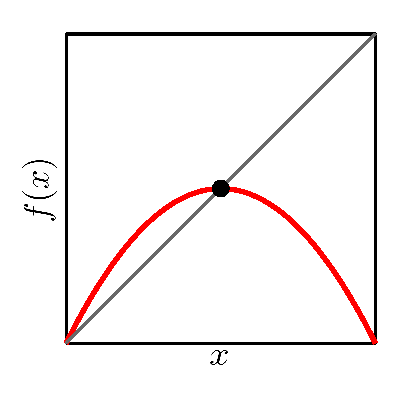
\includegraphics[width=\textwidth]{renormalization_1}
	\end{minipage}

	\vspace{1cm}
\end{frame}

\begin{frame}[t, c]{Logistic map}{Analysis : Renormalization}
	\begin{minipage}{.68\textwidth}
		\begin{itemize}
			\item Let us try to explain graphically this convergence of the sequence of \( \left\{ \mu_n \right\} \) as \( n \to \infty \).

			\medskip

			\item Compare the graph of \(f(x, \mu_1)\) and \(f^2(x, \mu_2)\) when \(x = 0.5\) is a superstable fixed point.

			\medskip

			\item In the vicinity of the superstable fixed point, these two graphs are very similar so that we have
			%
			\[
				f(x, \mu_1) \simeq \alpha f^2(\nicefrac{x}{\alpha}, \mu_2),
			\]
			%
			where \( \alpha < 0 \) (and \( \vert \alpha \vert > 1\) ) is a scaling parameter.
		\end{itemize}
	\end{minipage}%
	\hfill
	\begin{minipage}{.28\textwidth}
		\centering
		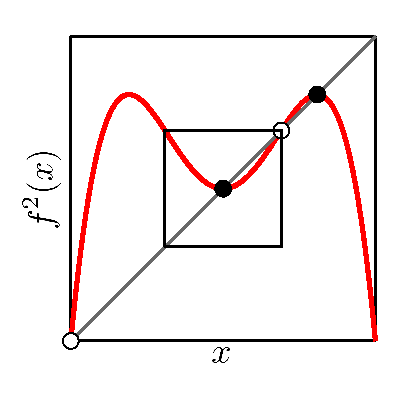
\includegraphics[width=\textwidth]{renormalization_2}
	\end{minipage}

	\vspace{1cm}
\end{frame}

\begin{frame}[t, c]{Logistic map}{Analysis : Renormalization}
	\begin{minipage}{.68\textwidth}
		\begin{itemize}
			\item Let us try to explain graphically this convergence of the sequence of \( \left\{ \mu_n \right\} \) as \( n \to \infty \).

			\medskip

			\item Compare the graph of \(f(x, \mu_0)\) and \(f^2(x, \mu_1)\) when \(x = 0.5\) is a superstable fixed point.

			\medskip

			\item In the vicinity of the superstable fixed point, these two graphs are very similar so that we have
			%
			\[
				f(x, \mu_0) \simeq \alpha f^2(\nicefrac{x}{\alpha}, \mu_1),
			\]
			%
			where \( \alpha < 0 \) (and \( \vert \alpha \vert > 1\) ) is a scaling parameter.
		\end{itemize}
	\end{minipage}%
	\hfill
	\begin{minipage}{.28\textwidth}
		\centering
		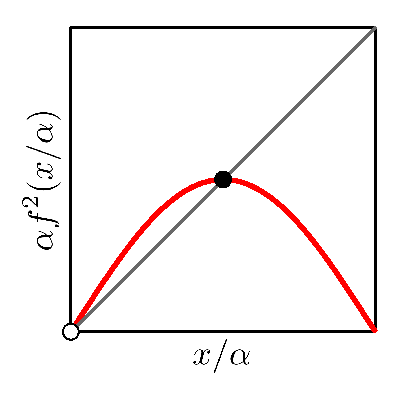
\includegraphics[width=\textwidth]{renormalization_3}
	\end{minipage}

	\vspace{1cm}
\end{frame}

\begin{frame}[t, c]{Logistic map}{Analysis : Renormalization}
	\begin{minipage}{.68\textwidth}
		\begin{itemize}
			\item \(f(x, \mu_1)\) has been \textbf{renormalized} by taking its second iterate, rescaling \(x \to \nicefrac{x}{\alpha}\) and shifting \( \mu \) to the next superstable value.

			\medskip

			\item We can keep this process going to renormalize \( f^2(x, \mu_1) \) to \( f^4(x, \mu_2) \) yielding
			%
			\[
				\begin{aligned}
					& f^2(x, \mu_1) \simeq \alpha f^4(\nicefrac{x}{\alpha^2}, \mu_2), \\
					& f(x, \mu_0) \simeq \alpha^2 f^4(\nicefrac{x}{\alpha^2}, \mu_2).
				\end{aligned}
			\]

			\item After n iterations, we have
			%
			\[
				f(x, \mu_0) \simeq \alpha^{n} f^{\left( 2^n \right)}(\nicefrac{x}{\alpha^n}, \mu_{n})
			\]
		\end{itemize}
	\end{minipage}%
	\hfill
	\begin{minipage}{.28\textwidth}
		\centering
		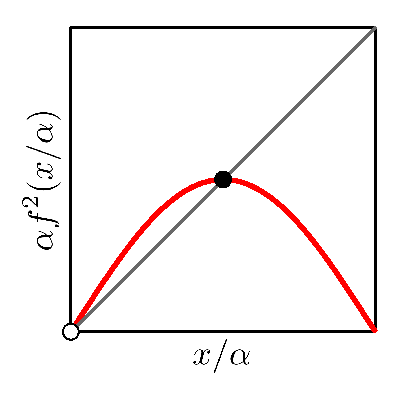
\includegraphics[width=\textwidth]{renormalization_3}
	\end{minipage}

	\vspace{1cm}
\end{frame}

\begin{frame}[t, c]{Logistic map}{Analysis : Renormalization}
	\begin{minipage}{.68\textwidth}
		\begin{itemize}
			\item It has been shown by Feigenbaum (1978) that
			%
			\[
				\lim_{n \to \infty} \alpha^n f^{(2^n)} \left( \frac{x}{\alpha^n}, \mu_n \right) = g_0(x),
			\]
			%
			where \( g_0(x) \) is a \textbf{universal function} with a superstable fixed point.

			\bigskip

			\item This limit exists only when the scale parameter \( \alpha \) is chosen appropriately, namely \( \alpha = -2.5029\ldots \)
		\end{itemize}
	\end{minipage}%
	\hfill
	\begin{minipage}{.28\textwidth}
		\centering
		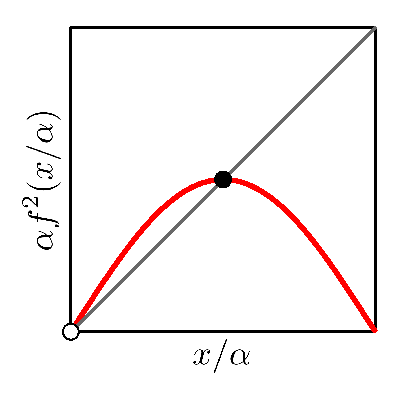
\includegraphics[width=\textwidth]{renormalization_3}
	\end{minipage}

	\vspace{1cm}
\end{frame}

\begin{frame}[t, c]{Logistic map}{Analysis : Renormalization}
	\begin{minipage}{.68\textwidth}
		\begin{itemize}
			\item To obtain the universal function \(g_1(x)\) with a superstable 2-cycle, start the renormalization process with \(f(x, \mu_1)\) instead of \(f(x, \mu_0)\) so that
			%
			\[
				\lim_{n \to \infty} \alpha^n f^{(2^n)} \left( \frac{x}{\alpha^n}, \mu_{n+1} \right) = g_1(x).
			\]
			%
			\item Of particular interest is the case where we start with \( \mu = \mu_{\infty} \) (at the onset of chaos). When then have
			%
			\[
				f(x, \mu_{\infty}) \simeq \alpha^2 f^2 \left( \frac{x}{\alpha}, \mu_{\infty} \right).
			\]
			%
			Note that we longer need to shift \( \mu \) to the next superstable value.
		\end{itemize}
	\end{minipage}%
	\hfill
	\begin{minipage}{.28\textwidth}
		\centering
		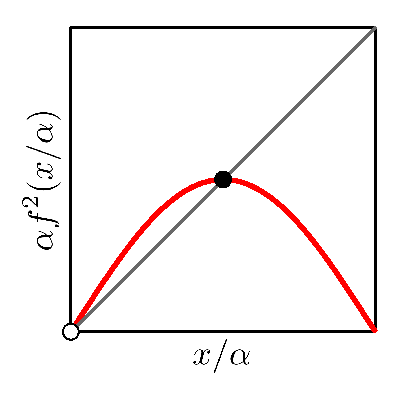
\includegraphics[width=\textwidth]{renormalization_3}
	\end{minipage}

	\vspace{1cm}
\end{frame}

\begin{frame}[t, c]{Logistic map}{Analysis : Renormalization}
	\begin{minipage}{.68\textwidth}
		\begin{itemize}
			\item The corresponding universal function \(g(x)\) satisfies the \textbf{functional equation}
			%
			\[
				g(x) = \alpha g^2 \left( \frac{x}{\alpha} \right)
			\]
			%
			with appropriate boundary conditions (e.g.\ \(g(0) = 1\), \(g^{\prime}(0) = 0\) and \(g^{\prime \prime}(0) < 0\) ).

			\medskip

			\item The scaling parameter \( \alpha \) is then given by
			%
			\[
				\alpha = \frac{1}{g(g(0))} = \frac{1}{g(1)}.
			\]
		\end{itemize}
	\end{minipage}%
	\hfill
	\begin{minipage}{.28\textwidth}
		\centering
		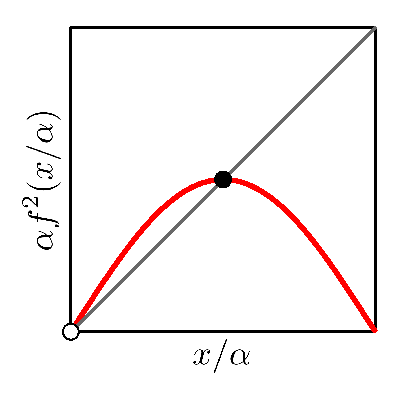
\includegraphics[width=\textwidth]{renormalization_3}
	\end{minipage}

	\vspace{1cm}
\end{frame}

\begin{frame}[t, c]{Logistic map}{Analysis : Renormalization}
	\begin{minipage}{.68\textwidth}
		\begin{itemize}
			\item No closed-form solutions have been found so far and we thus need to approximate \(g(x)\) using power series for instance, i.e.\
			%
			\[
				g(x) \simeq \sum_{k=0}^{n} a_i x^{2k}
			\]
			%
			for n sufficiently large.

			\item Feigenbaum used a seven-term expansion and found
			%
			\[
				c_2 \simeq -1.5276, \quad c_4 \simeq 0.1048
			\]
			%
			along with \( \alpha = -2.5029 \).

			\medskip

			\item The theory also explain the geometric factor \( \delta \) but it requires more sophisticated mathematics which are beyond the scope of this course.
		\end{itemize}
	\end{minipage}%
	\hfill
	\begin{minipage}{.28\textwidth}
		\centering
		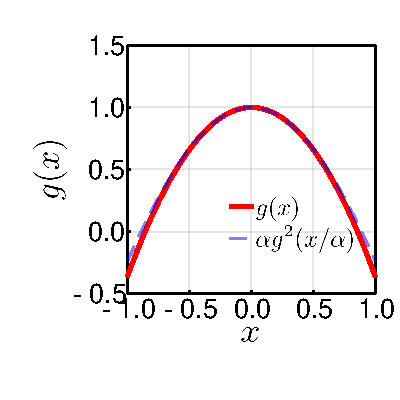
\includegraphics[width=\textwidth]{quadratic_functional_equation}
	\end{minipage}

	\vspace{1cm}
\end{frame}

\begin{frame}[t, c]{Logistic map}{Exercise : Renormalization}
	\begin{minipage}{.68\textwidth}
		\begin{itemize}
			\item Let us approximate \(g(x)\) as
			%
			\[
				g(x) \simeq 1 + a_1 x^2.
			\]

			\medskip

			\item Neglecting the quartic term, our functional equation becomes
			%
			\[
				1 + a_1 x^2 = \alpha ( 1 + a_1 ) + \frac{2 a_1^2 }{\alpha} x^2.
			\]

			\medskip

			\item We thus have
			%
			\[
				1 = \alpha ( 1 + a_1 ) \quad \text{and} \quad a_1 = \frac{\alpha}{2}.
			\]
		\end{itemize}
	\end{minipage}%
	\hfill
	\begin{minipage}{.28\textwidth}
		\centering
		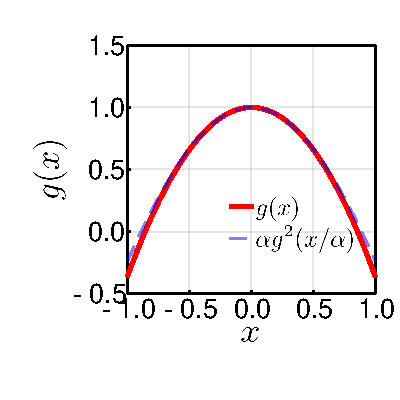
\includegraphics[width=\textwidth]{quadratic_functional_equation}
	\end{minipage}

	\vspace{1cm}
\end{frame}


\begin{frame}[t, c]{Logistic map}{Exercise : Renormalization}
	\begin{minipage}{.68\textwidth}
		\begin{itemize}
			\item Finally, using the condition \(g^{\prime \prime}(0) < 0\), we obtain
			%
			\[
				a_1 = \frac{-1 - \sqrt{3}}{2} \quad \text{and} \quad \alpha = -1 - \sqrt{3} \ (\simeq -2.732\ldots)
			\]

			\item Despite our two-term expansion of \(g(x)\), our approximate value of the scale parameter \( \alpha \) differs only by 9\% from its exact value.

			\bigskip

			\item Let us now look at this problem once more, but considering the bifurcation points rather than the superstable points.
		\end{itemize}
	\end{minipage}%
	\hfill
	\begin{minipage}{.28\textwidth}
		\centering
		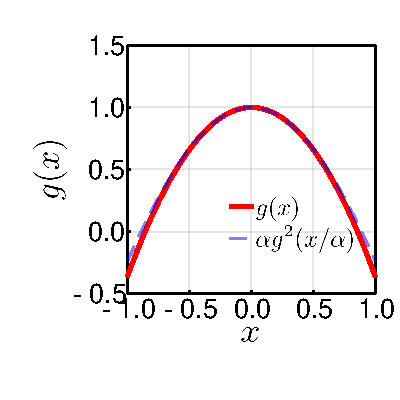
\includegraphics[width=\textwidth]{quadratic_functional_equation}
	\end{minipage}

	\vspace{1cm}
\end{frame}

\begin{frame}[t, c]{Logistic map}{Exercise : Renormalization}
	\begin{minipage}{.68\textwidth}
		\begin{itemize}
			\item Let us consider the system
			%
			\[
				x_{k+1} = f(x_k, \epsilon)
			\]
			%
			with \( f(x, \epsilon) = -\left( 1 + \epsilon \right) x_k + x_k^2 \).

			\medskip

			\item This system corresponds to a rescaling of the logistic map.

			\medskip

			\item In what follows, we will compute approximation of \( \alpha \) and \( \delta \), illustrating some of the basic ideas of renormalization.
		\end{itemize}
	\end{minipage}%
	\hfill
	\begin{minipage}{.28\textwidth}
		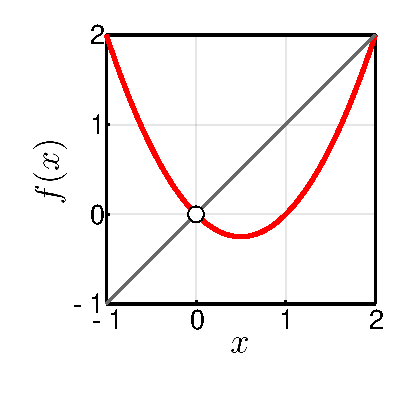
\includegraphics[width=\textwidth]{renormalization_normal_form}
	\end{minipage}

	\vspace{1cm}
\end{frame}

\begin{frame}[t, c]{Logistic map}{Exercise : Renormalization}
	\begin{minipage}{.68\textwidth}
		\begin{itemize}
			\item At \( \epsilon = 0 \), a flip bifurcation occurs. The fixed point \( x = 0 \) becomes unstable and a 2-cycle is created.

			\medskip

			\item Let us denote by \( p \) and \( q \) the two points of this cycle such that
			%
			\[
				p = -(1 + \epsilon) q + q^2 \quad \text{and} \quad q = -(1 + \epsilon) p + p^2.
			\]

			\item These points are thus fixed points of \(f^2(x) - x\) and are given by
			%
			\[
				p = \frac{\epsilon + \sqrt{\epsilon^2 + 4\epsilon}}{2} \quad \text{and} \quad q = \frac{\epsilon - \sqrt{\epsilon^2 + 4\epsilon}}{2}.
			\]
		\end{itemize}
	\end{minipage}%
	\hfill
	\begin{minipage}{.28\textwidth}
		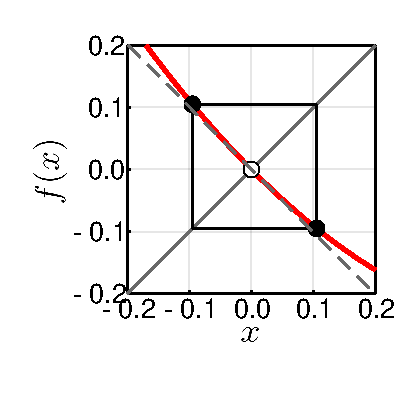
\includegraphics[width=\textwidth]{renormalization_flip_bifurcation}
	\end{minipage}

	\vspace{1cm}
\end{frame}

\begin{frame}[t, c]{Logistic map}{Exercise : Renormalization}
	\begin{minipage}{.68\textwidth}
		\begin{itemize}
			\item The dynamics of a perturbation \( \eta \) in the vicinity of \( p \) are governed by
			%
			\[
				p + \eta_{k+1} = f^2(p + \eta_k, \epsilon).
			\]

			\item Using a Taylor expansion, we have
			%
			\[
				\eta_{k+1} = \left( 1 - 4\epsilon - \epsilon^2 \right) \eta_k + C \eta_k^2 + \cdots,
			\]
			%
			where \( C = \nicefrac{\mathrm{d}^2 f(f(x))}{\mathrm{d}x^2} \) evaluated at \(x = p\).

			\medskip

			\item Introducing the scaled variable \( \tilde{x} = C\eta \), we obtain
			%
			\[
				\tilde{x}_{k+1} = \left( 1 - 4\epsilon - \epsilon^2 \right) \tilde{x}_k + \tilde{x}_k^2 + \cdots
			\]
			%
			Note that \( C \) plays the same rescaling role as \( \alpha \)!
		\end{itemize}
	\end{minipage}%
	\hfill
	\begin{minipage}{.28\textwidth}
		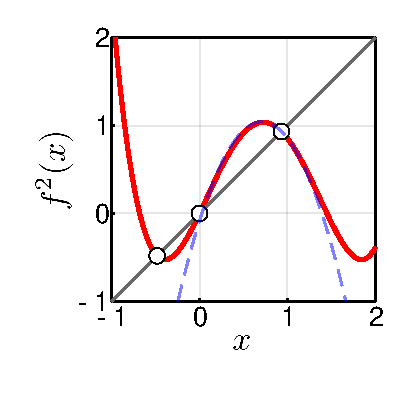
\includegraphics[width=\textwidth]{renormalization_2_cycle}
	\end{minipage}

	\vspace{1cm}
\end{frame}

\begin{frame}[t, c]{Logistic map}{Exercise : Renormalization}
	\begin{minipage}{.68\textwidth}
		\begin{itemize}
			\item Finally, introducing the renormalized parameter \( \tilde{\epsilon} = \epsilon^2 + 4\epsilon - 2 \), our system reads
			%
			\[
				\tilde{x}_{k+1} = -\left( 1 + \tilde{\epsilon} \right) \tilde{x}_k + \tilde{x}_k^2 + \cdots
			\]

			\item We thus recover a scaled version of our original system. It has been renormalized.

			\medskip

			\item When \( \tilde{\epsilon} = 0 \), the renormalized map undergoes a flip bifurcation.
			\begin{itemize}
				\item[\( \hookrightarrow \)] the 2-cycle of the original map loses stability and creates a 4-cycle.
			\end{itemize}

			\medskip

			\item We can then repeat this process \emph{ad infinitum}.
		\end{itemize}
	\end{minipage}%
	\hfill
	\begin{minipage}{.28\textwidth}
		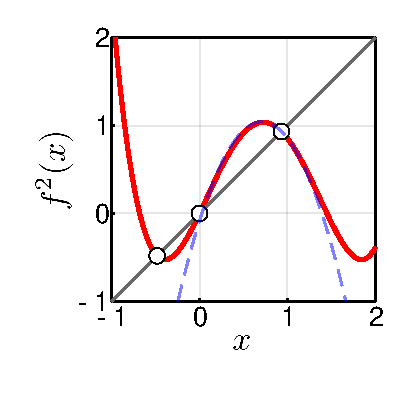
\includegraphics[width=\textwidth]{renormalization_2_cycle}
	\end{minipage}

	\vspace{1cm}
\end{frame}

\begin{frame}[t, c]{Logistic map}{Exercise : Renormalization}
	\begin{minipage}{.68\textwidth}
		\begin{itemize}
			\item It can easily be shown that \( \epsilon_k \) satisfies
			%
			\[
				\epsilon_{k-1} = \epsilon_k^2 + 4\epsilon_k -2,
			\]
			%
			or equivalently
			%
			\[
				\epsilon_{k} = -2 + \sqrt{6 + \epsilon_{k-1}}.
			\]
			%
			\item You can now easily show that
			%
			\[
				\begin{aligned}
					\epsilon^* & = \lim_{k\to\infty} \epsilon_k \\
					& = \frac{1}{2} \left( -3 + \sqrt{17} \right) \\
					& \simeq 0.56
				\end{aligned}
			\]

			\item At \( \epsilon = \epsilon^* \), a cycle of infinite period emerge. This is the onset of chaos.
		\end{itemize}
	\end{minipage}%
	\hfill
	\begin{minipage}{.28\textwidth}
		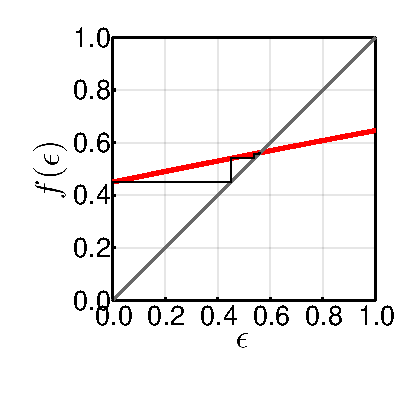
\includegraphics[width=\textwidth]{renormalization_epsilon_sequence}
	\end{minipage}

	\vspace{1cm}
\end{frame}

\begin{frame}[t, c]{Logistic map}{Exercise : Renormalization}
	\begin{minipage}{.68\textwidth}
		\begin{itemize}
			\item Recalling that \( \epsilon = 0 \iff \mu = 3 \) for the logistic map (i.e.\ creation of the 2-cycle), we thus predict \( \mu_{\infty} = 3.56 \) while numerical computations show \( \mu_{\infty} = 3.5699\ldots \)

			\medskip

			\item For \( k \gg 1 \), the sequence \( \{ \epsilon_k \} \) converges toward \( \epsilon^* \) at a rate given by the Feigenbaum constant \( \delta \), hence
			%
			\[
				\begin{aligned}
					\delta & = \lim_{k \to \infty} \frac{\epsilon_{k-1} - \epsilon^*}{\epsilon_{k} - \epsilon^*} \\
					& = \frac{\mathrm{d} \epsilon_{k-1}}{\mathrm{d}\epsilon_k}\bigg\lvert_{\epsilon=\epsilon^*} \\
					& = 1 + \sqrt{17} \simeq 5.12.
				\end{aligned}
			\]

			\item Our estimate is only 10\% larger than the true value of \( \delta \).
		\end{itemize}
	\end{minipage}%
	\hfill
	\begin{minipage}{.28\textwidth}
		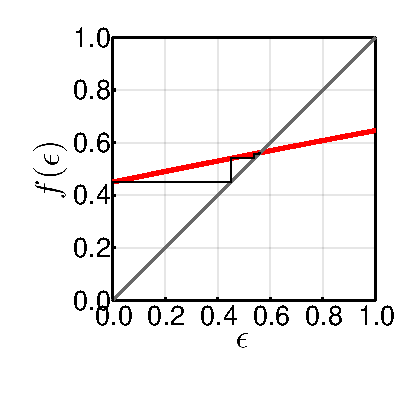
\includegraphics[width=\textwidth]{renormalization_epsilon_sequence}
	\end{minipage}

	\vspace{1cm}
\end{frame}

\begin{frame}[t, c]{Logistic map}{Into the chaos}
	\begin{minipage}{.68\textwidth}
		\begin{itemize}
			\item At \( \epsilon = \epsilon^* \), a cycle of infinite period emerge. This is the onset of chaos.

			\bigskip

			\item Although renormalization theory was helpful to determine the onset of chaos, it provides no information about how to characterize chaotic dynamics (for \( \mu > \mu_{\infty} \)).

			\bigskip

			\item We need to introduce new mathematical concepts!

		\end{itemize}
	\end{minipage}%
	\hfill
	\begin{minipage}{.28\textwidth}
		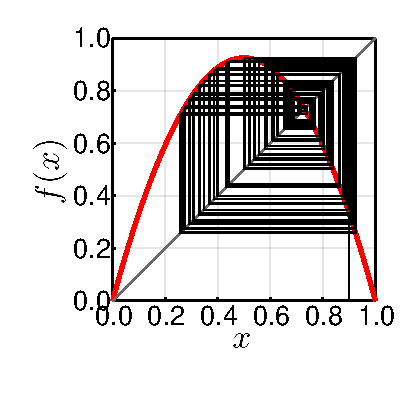
\includegraphics[width=\textwidth]{into_the_chaos}
	\end{minipage}

	\vspace{1cm}
\end{frame}

\begin{frame}[t, c]{Logistic map}{Analysis : Lyapunov exponent}
	\begin{minipage}{.58\textwidth}
		\centering
		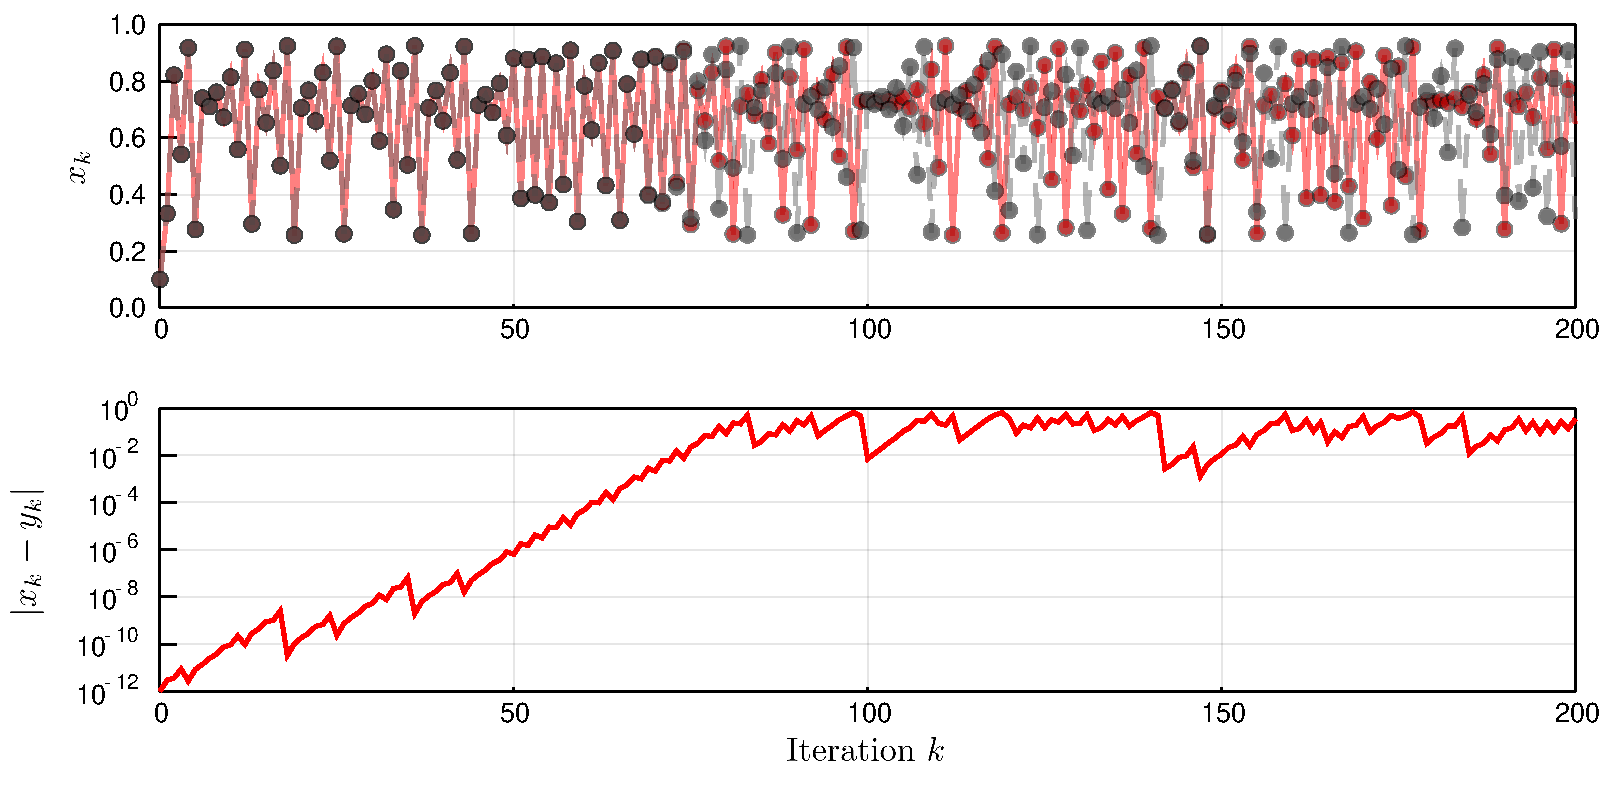
\includegraphics[width=\textwidth]{lyapunov_time_series}
	\end{minipage}%
	\hfill
	\begin{minipage}{.38\textwidth}
		\begin{itemize}
			\item In the chaotic regime, the system exhibits \textbf{sensitive dependence on the initial condition}.

			\medskip

			\item Two nearby trajectories eventually diverge exponentially fast.

			\medskip

			\item The rate at which they diverge is given by the so-called \textbf{Lyapunov exponent}.
		\end{itemize}
	\end{minipage}

	\vspace{1cm}
\end{frame}

\begin{frame}[t, c]{Logistic map}{Analysis : Lyapunov exponent}
	\begin{minipage}{.58\textwidth}
		\begin{itemize}
			\item Consider two initial points given by \( x_0 \) and \( x_0 + \delta_0 \).
			After n iterations, we have \( \vert \delta_n \vert \simeq \vert \delta_0 \vert e^{\lambda n} \) where \( \lambda \) is the Lyapunov exponent.
			\begin{itemize}
				\item[\( \hookrightarrow \)] \( \lambda > 0 \) is the signature of chaos.
			\end{itemize}

			\item A more precise and computational useful formula can be derived by noting that \( \delta_n = f^n(x_0 + \delta_0)  - f^n(x_0) \). Then
			%
			\[
				\begin{aligned}
					\lambda & = \frac{1}{n} \log \Big\vert \frac{\delta_n}{\delta_0} \Big\vert \\
					& = \frac{1}{n} \log \Big\vert \frac{f^n(x_0 + \delta_0) - f^n(x_0)}{\delta_0} \Big\vert \\
					& = \frac{1}{n} \log \vert \left(f^n\right)^{\prime}(x_0) \vert.
				\end{aligned}
			\]
			when \( \delta_0 \to 0 \).
		\end{itemize}
	\end{minipage}%
	\hfill
	\begin{minipage}{.38\textwidth}
		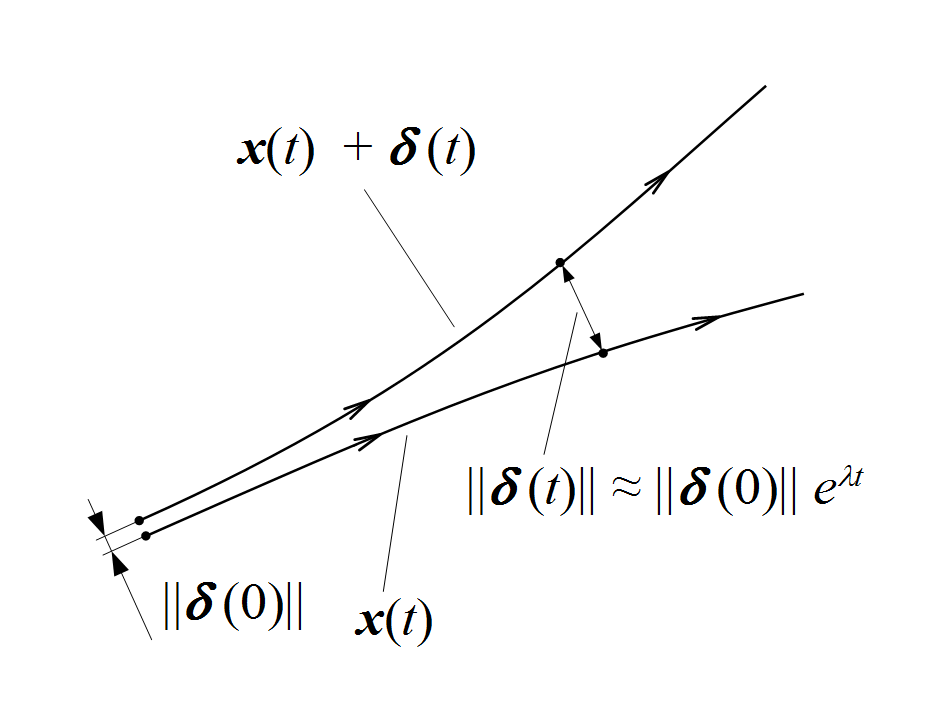
\includegraphics[width=\textwidth]{lyapunov}
	\end{minipage}

	\vspace{1cm}
\end{frame}

\begin{frame}[t, c]{Logistic map}{Analysis : Lyapunov exponent}
	\begin{minipage}{.58\textwidth}
		\begin{itemize}
			\item Noting that \( \left( f^n \right)^{\prime}(x_0) = \prod_{i=0}^{n-1} f^{\prime}(x_i)\), we finally have
			%
			\[
				\lambda = \frac{1}{n} \sum_{i=0}^{n-1} \log \vert f^{\prime}(x_i) \vert.
			\]

			\item When \(n \to \infty\), we define the limit to be the \textbf{Lyapunov exponent} for the orbit starting at \(x_0\)
			%
			\[
				\lambda = \displaystyle \lim_{n \to \infty} \frac{1}{n} \sum_{i=0}^{n-1} \log \vert f^{\prime}(x_i) \vert.
			\]

			\item Although \( \lambda \) appears to depend on \( x_0 \), it is actually the same for \( x_0 \) in the basin of attraction of a given attractor.
		\end{itemize}
	\end{minipage}%
	\hfill
	\begin{minipage}{.38\textwidth}
		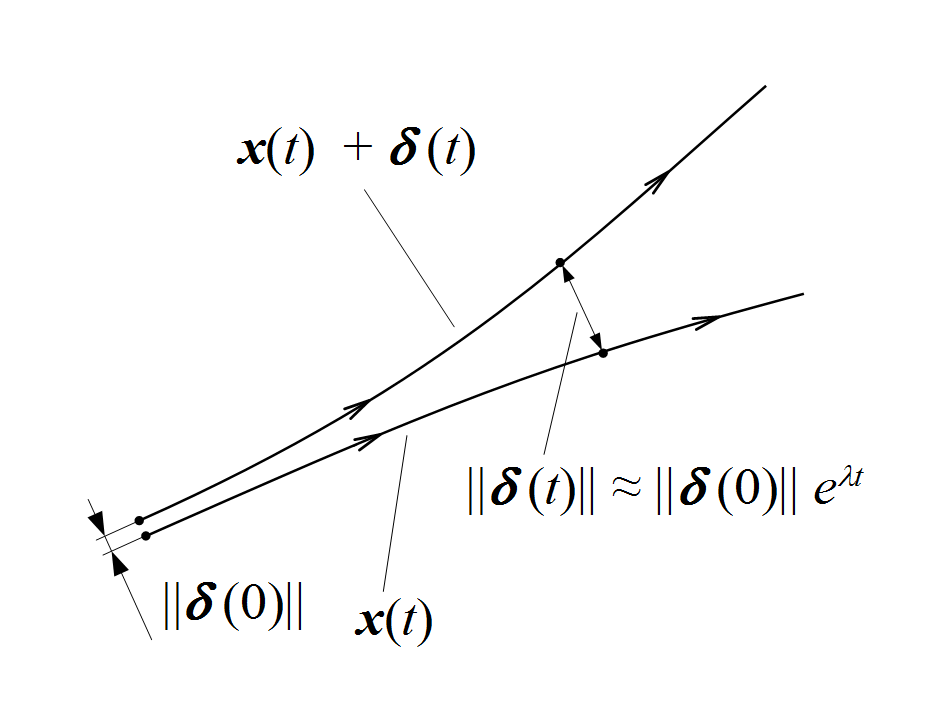
\includegraphics[width=\textwidth]{lyapunov}
	\end{minipage}

	\vspace{1cm}
\end{frame}

\begin{frame}[t, c]{Logistic map}{Analysis : Lyapunov exponent}

	\begin{itemize}
		\item When the system is stable, \( \lambda < 0 \). At each bifurcation point, we have \( \lambda = 0 \), while \( \lambda > 0 \) once the system is chaotic.
	\end{itemize}

	\medskip

	\centering
	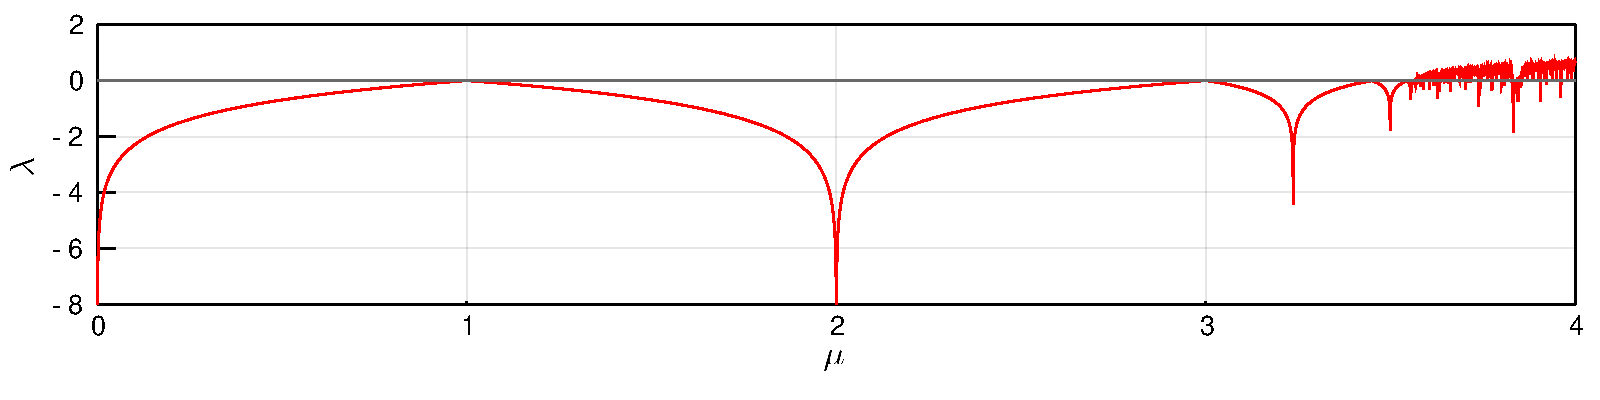
\includegraphics[width=\textwidth]{lyapunov_exponents}

	\vspace{1cm}
\end{frame}

\begin{frame}[t, c]{Logistic map}{Analysis : Periodic windows}
	\begin{minipage}{.68\textwidth}
		\begin{itemize}
			\item Zooming in the range \(3.5 \leq \lambda \leq 4 \), small windows of non-chaotic regimes can be seen.

			\bigskip

			\item These correspond to so-called \textbf{periodic windows} over which the system exhibits \(3 \cdot 2^n\)-cycles, \(5 \cdot 2^n\)-cycles, etc.

			\bigskip

			\item In what follows, we will look more closely at what happens in the range \( 3.8 \leq \lambda \leq 3.9 \) during which the system exhibits such \(3 \cdot 2^n\)-cycles.
		\end{itemize}
	\end{minipage}%
	\hfill
	\begin{minipage}{.28\textwidth}
		\centering
		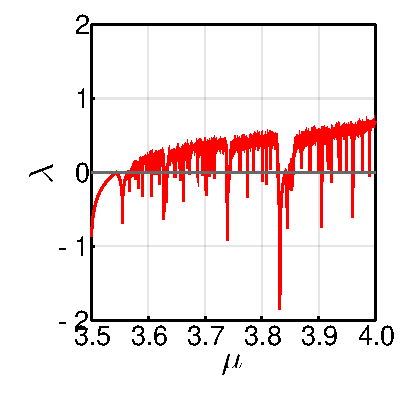
\includegraphics[width=\textwidth]{lyapunov_exponents_zoom}
	\end{minipage}

	\vspace{1cm}
\end{frame}


\begin{frame}[t, c]{Logistic map}{Analysis : Periodic windows}
	\begin{minipage}{.68\textwidth}
		\begin{itemize}
			\item Zooming in the range \(3.5 \leq \lambda \leq 4 \), small windows of non-chaotic regimes can be seen.

			\bigskip

			\item These correspond to so-called \textbf{periodic windows} over which the system exhibits \(3 \cdot 2^n\)-cycles, \(5 \cdot 2^n\)-cycles, etc.

			\bigskip

			\item In what follows, we will look more closely at what happens in the range \( 3.8 \leq \lambda \leq 3.9 \) during which the system exhibits such \(3 \cdot 2^n\)-cycles.
		\end{itemize}
	\end{minipage}%
	\hfill
	\begin{minipage}{.28\textwidth}
		\centering
		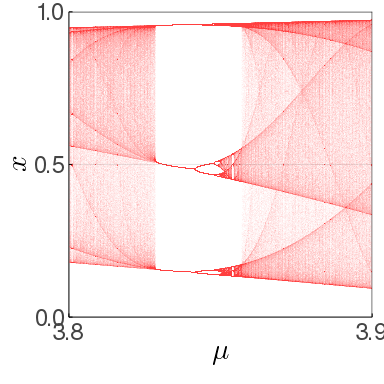
\includegraphics[width=\textwidth]{orbit_diagram_b}
	\end{minipage}

	\vspace{1cm}
\end{frame}

\begin{frame}[t, c]{Logistic map}{Analysis : \( 3 \cdot 2^n \)-cycles}
	\begin{minipage}{.68\textwidth}
		\begin{itemize}
			\item At \( \lambda = 1 + \sqrt{8} \), a \textbf{tangent bifurcation} (or saddle-node bifurcation) occurs, giving rise to a 3-cycle.

			\medskip

			\item Further increasing \( \lambda \), a new subharmonic cascade happens giving rise to a sequence of \(3 \cdot 2^n\)-cycles.
		\end{itemize}

		\bigskip

		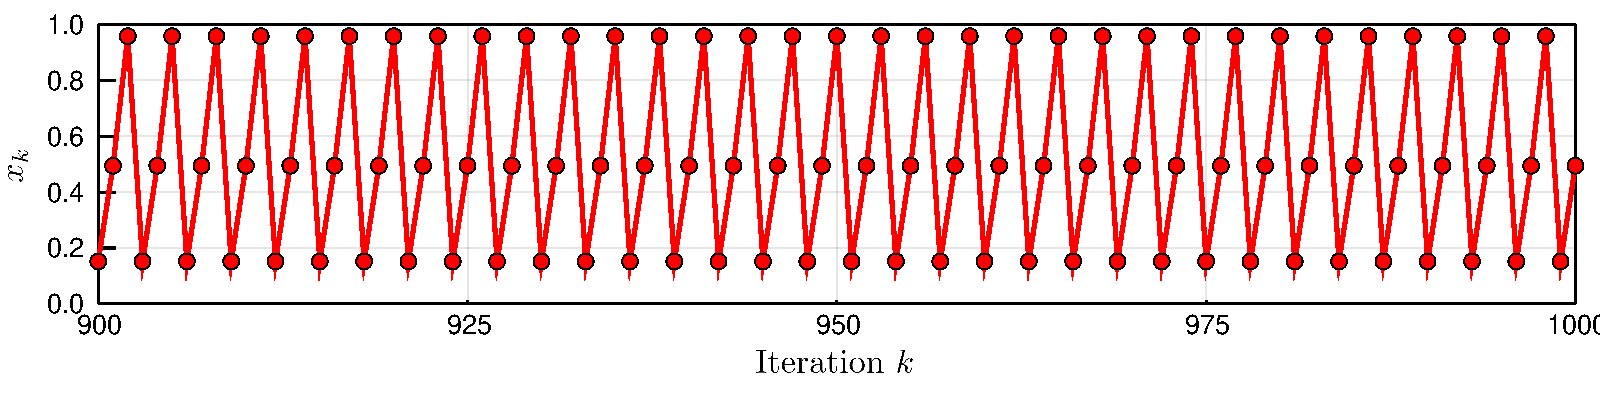
\includegraphics[width=\textwidth]{cycle_3_time_series}
	\end{minipage}%
	\hfill
	\begin{minipage}{.28\textwidth}
		\centering
		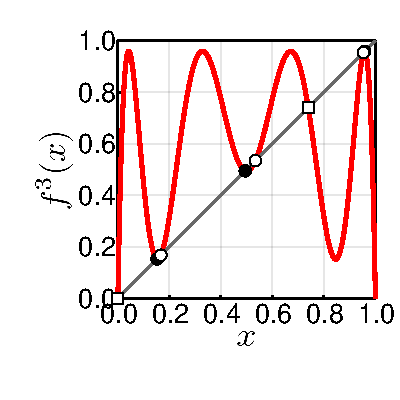
\includegraphics[width=\textwidth]{cycle_3_creation}
	\end{minipage}

	\vspace{1cm}
\end{frame}

\begin{frame}[t, c]{Logistic map}{Analysis : Intermittency}
	\begin{minipage}{.68\textwidth}
		\begin{itemize}
			\item For \( \lambda \) slightly smaller than \(1 + \sqrt{8} \), the system exhibits almost periodic dynamics separated by random bursts of chaos.
			\begin{itemize}
				\item[\( \hookrightarrow \)] The system sees the "ghost" of the 3-cycle.
			\end{itemize}

			\item It is better understood by looking at the cobweb and zooming in the vicinity of the ghost of one of the fixed points of \(f^{3}(x)-x\).
		\end{itemize}

		\bigskip

		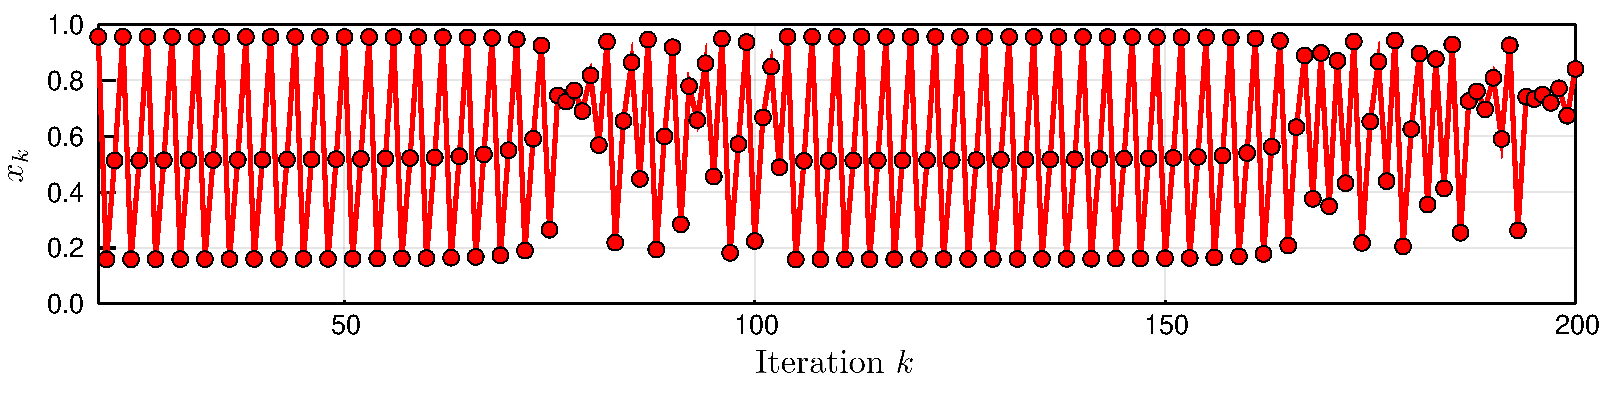
\includegraphics[width=\textwidth]{cycle_3_intermittency_time_series}
	\end{minipage}%
	\hfill
	\begin{minipage}{.28\textwidth}
		\centering
		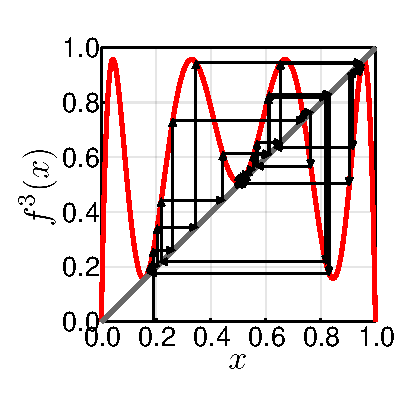
\includegraphics[width=\textwidth]{cycle_3_intermittency}
	\end{minipage}

	\vspace{1cm}
\end{frame}

\begin{frame}[t, c]{Logistic map}{Analysis : Intermittency}
	\begin{minipage}{.68\textwidth}
		\begin{itemize}
			\item For \( \lambda \) slightly smaller than \(1 + \sqrt{8} \), the system exhibits almost periodic dynamics separated by random bursts of chaos.
			\begin{itemize}
				\item[\( \hookrightarrow \)] The system sees the "ghost" of the 3-cycle.
			\end{itemize}

			\item It is better understood by looking at the cobweb and zooming in the vicinity of the ghost of one of the fixed points of \(f^{3}(x)-x\).
		\end{itemize}

		\bigskip

		\includegraphics[width=\textwidth]{cycle_3_intermittency_time_series}
	\end{minipage}%
	\hfill
	\begin{minipage}{.28\textwidth}
		\includegraphics[width=\textwidth]{cycle_3_intermittency_close_up}

		{\small
			Type-I intermittency according to Pomeau-Manneville.
		}
	\end{minipage}

	\vspace{1cm}
\end{frame}

\begin{frame}[t, c]{Universality of the subharmonic cascade}{Discrete system : Sine map}
	\begin{minipage}{.48\textwidth}
		\begin{itemize}
			\item The sine map is another one-dimensional unimodal map defined as
			%
			\[
				x_{k+1} = \mu \sin \left( \pi x_k \right).
			\]

			\medskip

			\item Its orbit diagram is suprisingly similar to that of the logistic map.
			\begin{itemize}
				\item[\( \hookrightarrow \)] Can be explained by the renormalization theory.
			\end{itemize}
		\end{itemize}
	\end{minipage}%
	\hfill
	\begin{minipage}{.48\textwidth}
		\includegraphics[width=\textwidth]{sine_map_orbit_diagram}
	\end{minipage}

	\vspace{1cm}
\end{frame}

\begin{frame}[t, c]{Universality of the subharmonic cascade}{Continuous system : R\"ossler system}
	\begin{minipage}{.48\textwidth}
		\begin{itemize}
			\item The R\"ossler system is a continuous-time three-dimensional system given by
			%
			\[
				\begin{aligned}
					& \dot{x} = -y - z \\
					& \dot{y} = x + ay \\
					& \dot{z} = b + z \left( x - c \right).
				\end{aligned}
			\]

			\item Tts orbit diagram (for \( a = 0.2 \) and \( c = 5.7 \)) is also similar to that of the logistic map.

			\medskip

			\item The mechanisms causing the emergence of chaos in the logistic map also exist here.
			\begin{itemize}
				\item[\( \hookrightarrow \)] This will be the subject of another course.
			\end{itemize}
		\end{itemize}
	\end{minipage}%
	\hfill
	\begin{minipage}{.48\textwidth}
		\includegraphics[width=\textwidth]{rossler_orbit_diagram}
	\end{minipage}

	\vspace{1cm}
\end{frame}

\thanksframe

\end{document}
